%\documentclass[prb,twocolumn,showpacs,aps,floats,floatfix,superscriptaddress]{revtex4}
%\documentclass[prb,showpacs,aps,floats,floatfix,superscriptaddress]{revtex4}
%\documentclass{article}
%\usepackage{epsfig,amsmath,amssymb,array,dcolumn,subfigure,rotating}

\documentclass[onecolumn,letterpaper,amsmath,amssymb,floatfix,aps,superscriptaddress]{revtex4}
%\documentclass[a4paper]{article}
\usepackage{graphicx}% Include figure files
\usepackage{dcolumn}% Align table columns on decimal point
\usepackage{bm}% bold math
\usepackage{epsfig,color}
\usepackage{wrapfig}


\usepackage{epsfig}

\def\ul#1#2{\textstyle{\frac#1#2}}
\def\rot{\operatorname{rot}}
\def\diver{\operatorname{div}}
\def\bnabla{\mbox{\boldmath $\nabla $}}
\def\bepsilon{\mbox{\boldmath $\epsilon $}}

\begin{document}

\title{\bf Hamaker coefficents for two identical anisotropic cylinder at all separations
A comparison of Gecko Hamaker and Python results} 

\author{J. Hopkins}
    
\begin{abstract}
Dan sent some data, I made A's. He generated A's from GH. I plotted both results for comparison. They should agree. They don't.
\end{abstract}

\maketitle        

\section{Imaginary part of the dielectric response function and Anisotropy metric}

The dielectric response functions are evaluated at imaginary frequencies, 
thus $\epsilon_{\parallel,\perp} = \epsilon_{\parallel,\perp}(i \omega)$. $\epsilon_{\parallel,\perp}(i \omega)$ is referred to as the London - van der Waals 
transform of the response function $\epsilon_{\parallel,\perp}(\omega)$ and is given by the Kramers - Kronig relations. It is strictly a real, monotonically 
decaying function of $\omega$. 
%%%%%%%%%EPS2 and Aiz%%%%%%%%%%%%%%%%%%%%%%%%%%%%%%%%%%%%%%%%%%%%%%%%
\begin{figure*}[t!]
\begin{center}
\begin{minipage}[b]{0.40\textwidth}
\begin{center}
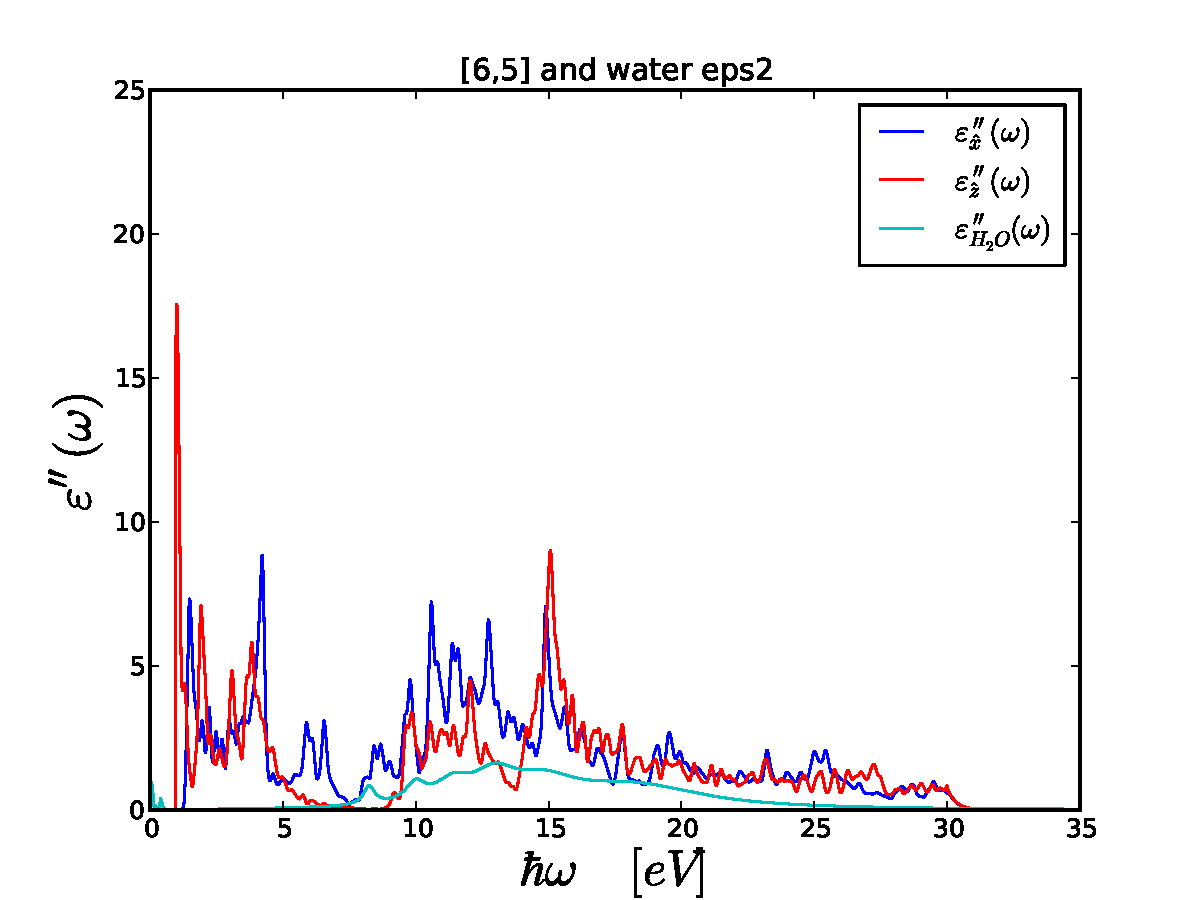
\includegraphics[width=1.2\textwidth]{prop_plots/65w65_eps2.pdf} (a)
\end{center}
\end{minipage}
\hskip 43pt
\begin{minipage}[b]{0.40\textwidth}
\begin{center}
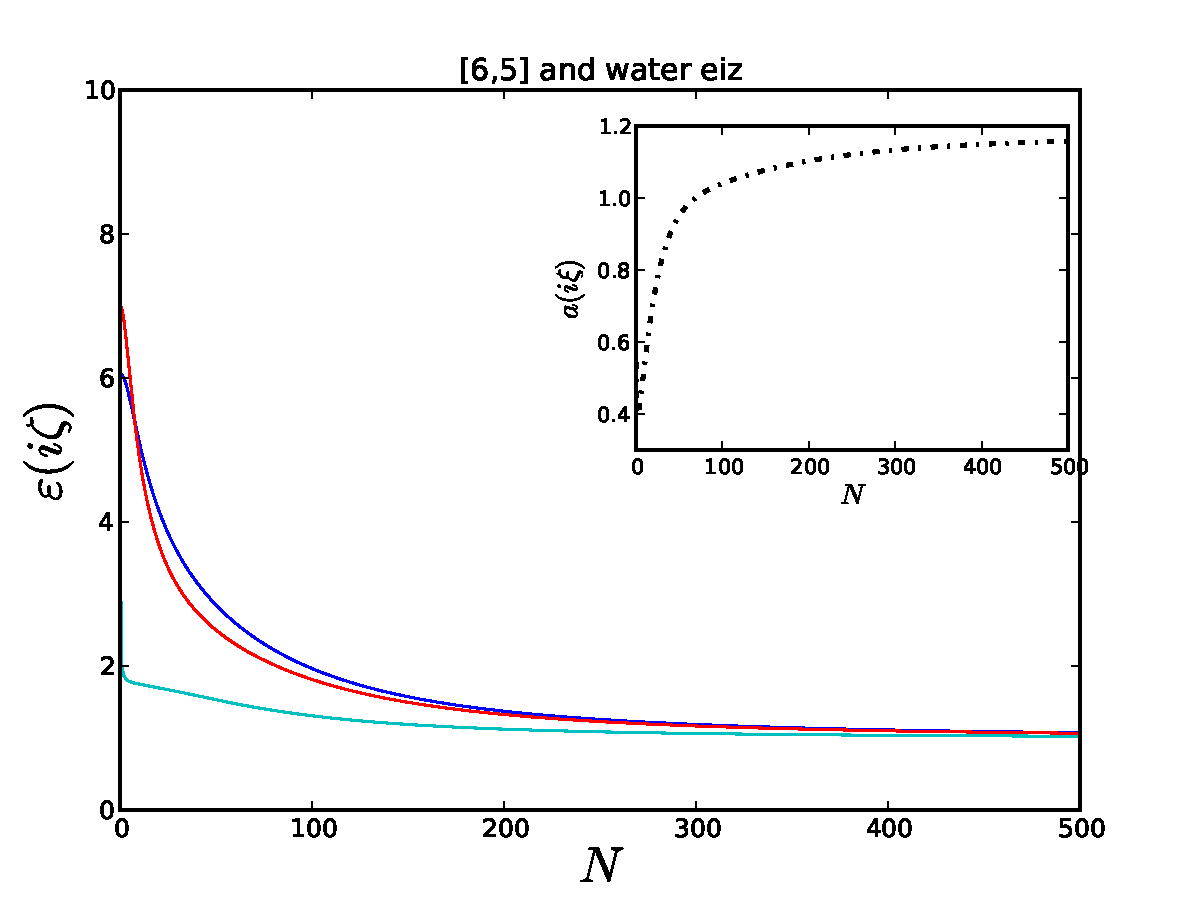
\includegraphics[width=1.2\textwidth]{prop_plots/65w65_eiz.pdf} (b)
\end{center}
\end{minipage}
\caption{Full result using Eqs.\ref{pars-31},\ref{pars-31-g} (a) Anisotropic response functions for CG-10 DNA and water. The DNA response functions in the x and y directions were used as perpendicular and parallel inputs, respectively.  CG-10 and water eps2 data was provided by Dan Dryden. CG-10 data scales Wai-Yim's calculations by 4.94 and is assumed to include Na (more info in Dan Dryden email sent to us on Nov. 8, 2013).  Water data was built from lorentz oscillators R.H.French,J.Amer.Ceram Soc.,83,9,2117-46(2000), H.D.Ackler, et al,J.Coll.Interface Sci.179,46.
(b) Anisotropy metric $a_{1,2}(i\zeta_n)$ using Eq.\ref{eq:adef}, compares the anisotropy of the  cylinders (DNA) to their intervening material, water for the terms contruting to the Matsubara sum.}
\label{eiz65}
\end{center}
\end{figure*} 

%%%%%%%%%EPS2 and Aiz%%%%%%%%%%%%%%%%%%%%%%%%%%%%%%%%%%%%%%%%%%%%%%%%
\begin{figure*}[t!]
\begin{center}
\begin{minipage}[b]{0.40\textwidth}
\begin{center}
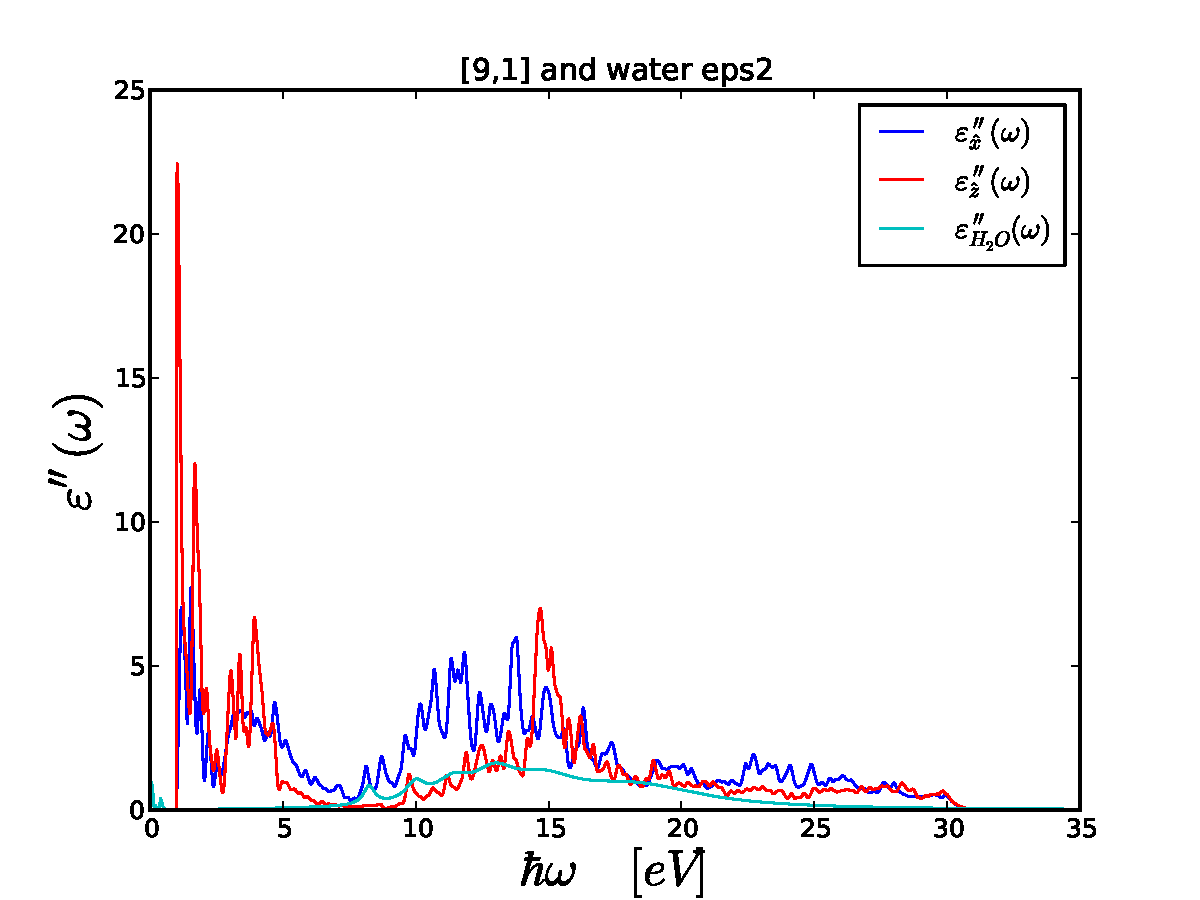
\includegraphics[width=1.2\textwidth]{prop_plots/91w91_eps2.pdf} (a)
\end{center}
\end{minipage}
\hskip 43pt
\begin{minipage}[b]{0.40\textwidth}
\begin{center}
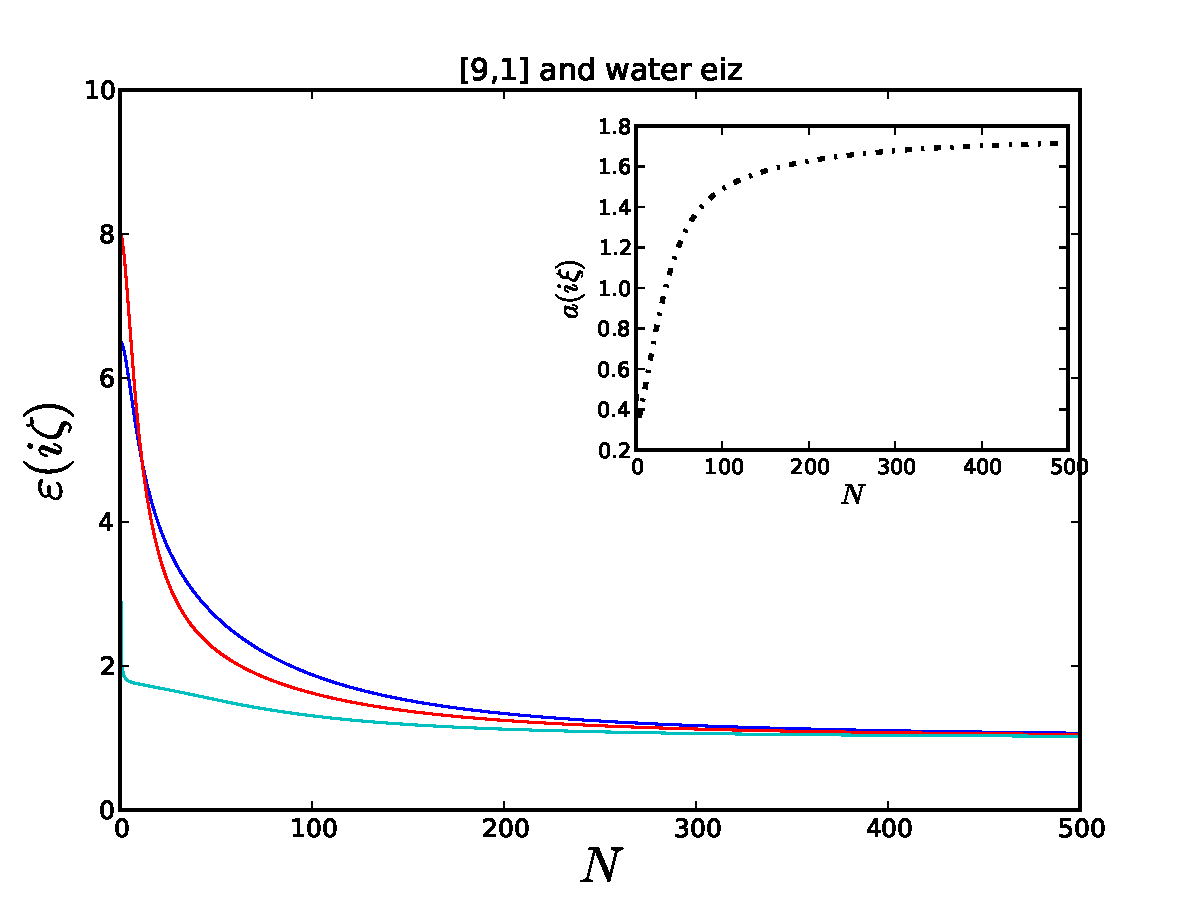
\includegraphics[width=1.2\textwidth]{prop_plots/91w91_eiz.pdf} (b)
\end{center}
\end{minipage}
\caption{Full result using Eqs.\ref{pars-31},\ref{pars-31-g} (a) Anisotropic response functions for CG-10 DNA and water. The DNA response functions in the x and y directions were used as perpendicular and parallel inputs, respectively.  CG-10 and water eps2 data was provided by Dan Dryden. CG-10 data scales Wai-Yim's calculations by 4.94 and is assumed to include Na (more info in Dan Dryden email sent to us on Nov. 8, 2013).  Water data was built from lorentz oscillators R.H.French,J.Amer.Ceram Soc.,83,9,2117-46(2000), H.D.Ackler, et al,J.Coll.Interface Sci.179,46.
(b) Anisotropy metric $a_{1,2}(i\zeta_n)$ using Eq.\ref{eq:adef}, compares the anisotropy of the  cylinders (DNA) to their intervening material, water for the terms contruting to the Matsubara sum.}
\label{eiz91}
\end{center}
\end{figure*} 

%%%%%%%%%EPS2 and Aiz%%%%%%%%%%%%%%%%%%%%%%%%%%%%%%%%%%%%%%%%%%%%%%%%
\begin{figure*}[t!]
\begin{center}
\begin{minipage}[b]{0.40\textwidth}
\begin{center}
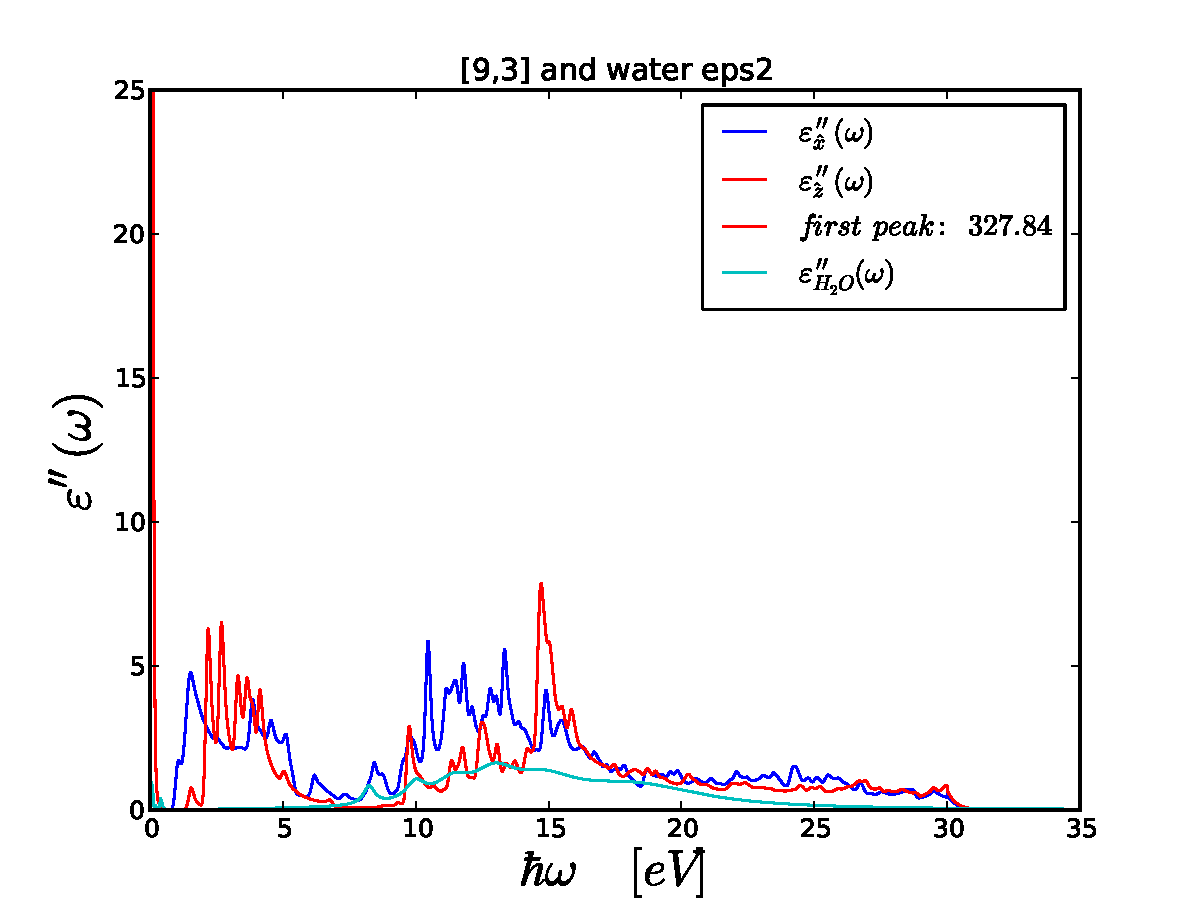
\includegraphics[width=1.2\textwidth]{prop_plots/93w93_eps2.pdf} (a)
\end{center}
\end{minipage}
\hskip 43pt
\begin{minipage}[b]{0.40\textwidth}
\begin{center}
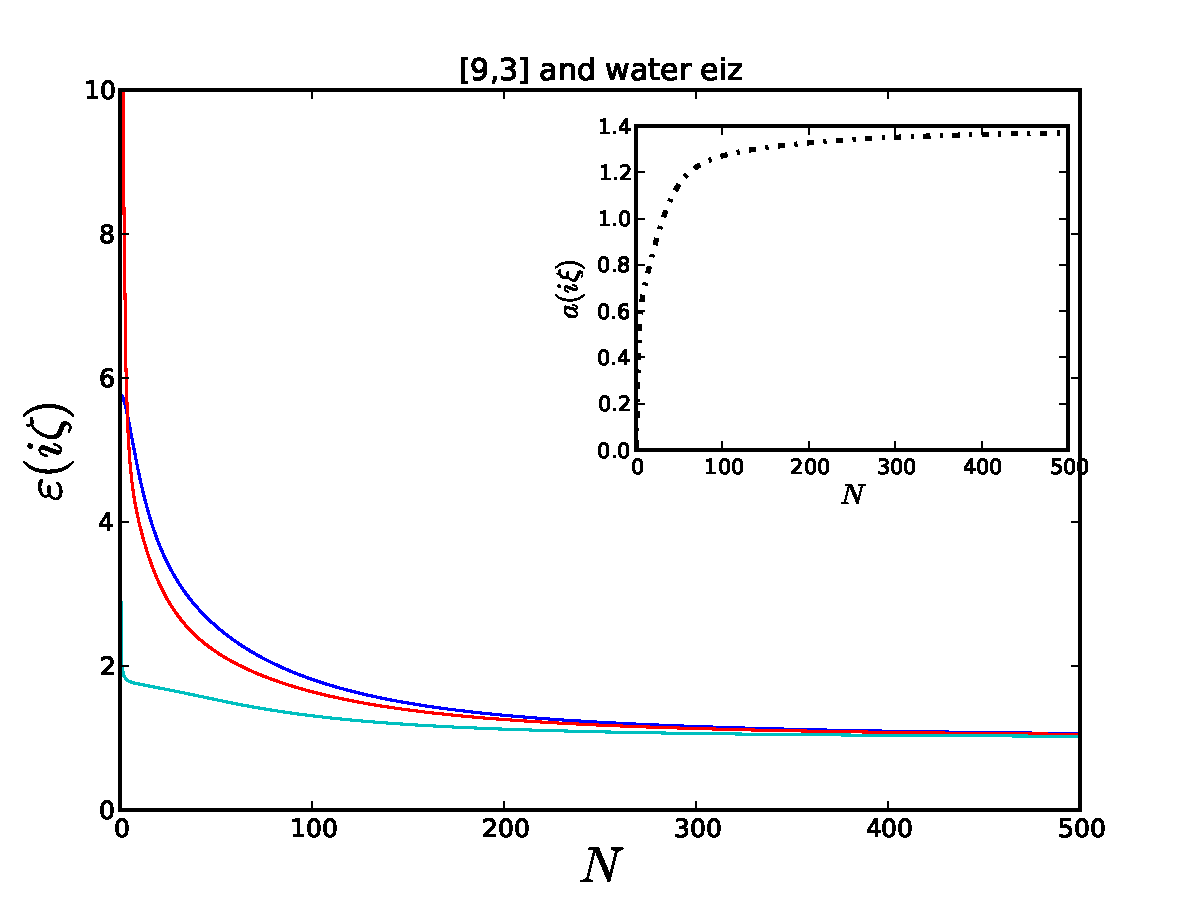
\includegraphics[width=1.2\textwidth]{prop_plots/93w93_eiz.pdf} (b)
\end{center}
\end{minipage}
\caption{Full result using Eqs.\ref{pars-31},\ref{pars-31-g} (a) Anisotropic response functions for CG-10 DNA and water. The DNA response functions in the x and y directions were used as perpendicular and parallel inputs, respectively.  CG-10 and water eps2 data was provided by Dan Dryden. CG-10 data scales Wai-Yim's calculations by 4.94 and is assumed to include Na (more info in Dan Dryden email sent to us on Nov. 8, 2013).  Water data was built from lorentz oscillators R.H.French,J.Amer.Ceram Soc.,83,9,2117-46(2000), H.D.Ackler, et al,J.Coll.Interface Sci.179,46.
(b) Anisotropy metric $a_{1,2}(i\zeta_n)$ using Eq.\ref{eq:adef}, compares the anisotropy of the  cylinders (DNA) to their intervening material, water for the terms contruting to the Matsubara sum.}
\label{eiz93}
\end{center}
\end{figure*} 

%%%%%%%%%EPS2 and Aiz%%%%%%%%%%%%%%%%%%%%%%%%%%%%%%%%%%%%%%%%%%%%%%%%
\begin{figure*}[t!]
\begin{center}
\begin{minipage}[b]{0.40\textwidth}
\begin{center}
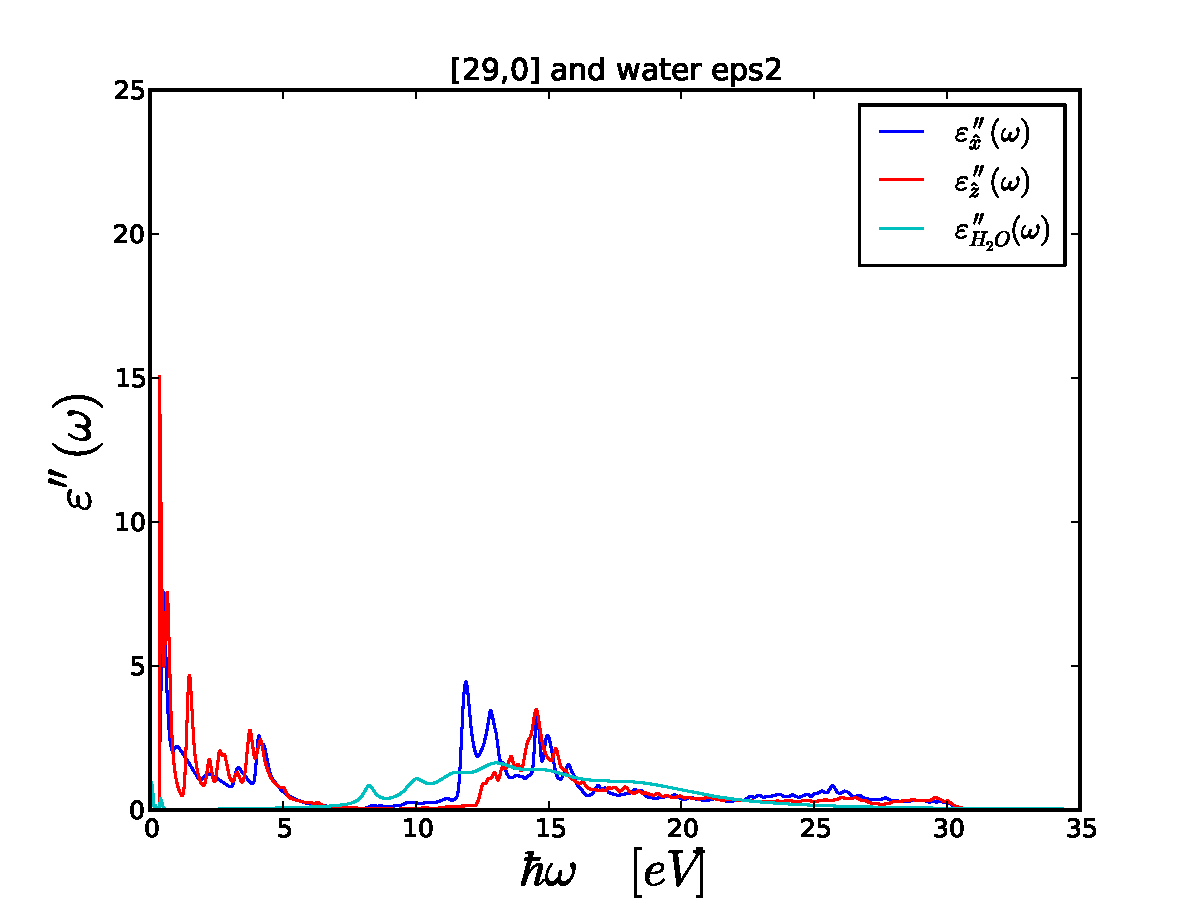
\includegraphics[width=1.2\textwidth]{prop_plots/290w290_eps2.pdf} (a)
\end{center}
\end{minipage}
\hskip 43pt
\begin{minipage}[b]{0.40\textwidth}
\begin{center}
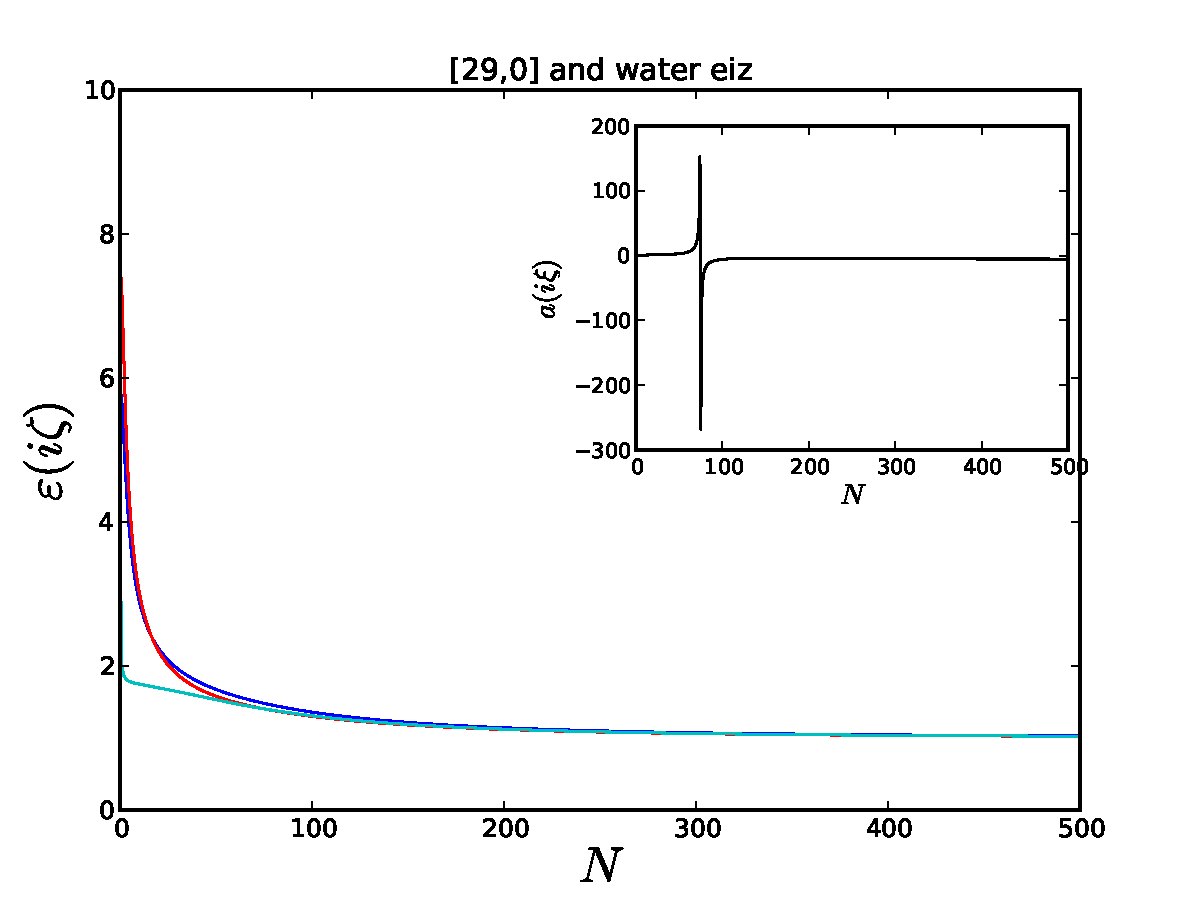
\includegraphics[width=1.2\textwidth]{prop_plots/290w290_eiz.pdf} (b)
\end{center}
\end{minipage}
\caption{Full result using Eqs.\ref{pars-31},\ref{pars-31-g} (a) Anisotropic response functions for CG-10 DNA and water. The DNA response functions in the x and y directions were used as perpendicular and parallel inputs, respectively.  CG-10 and water eps2 data was provided by Dan Dryden. CG-10 data scales Wai-Yim's calculations by 4.94 and is assumed to include Na (more info in Dan Dryden email sent to us on Nov. 8, 2013).  Water data was built from lorentz oscillators R.H.French,J.Amer.Ceram Soc.,83,9,2117-46(2000), H.D.Ackler, et al,J.Coll.Interface Sci.179,46.
(b) Anisotropy metric $a_{1,2}(i\zeta_n)$ using Eq.\ref{eq:adef}, compares the anisotropy of the  cylinders (DNA) to their intervening material, water for the terms contruting to the Matsubara sum.}
\label{eiz290}
\end{center}
\end{figure*} 

\section{Anisotropy Metric}
The ratios between the relative anisotropy measures (Eq. \ref{anisoind}) defined as 
\begin{equation}
a = \frac{2 \Delta_{\perp}}{\Delta_{\parallel}} = 2 \frac{({\epsilon^{c}}_{\perp}-\epsilon_{m}) \epsilon_{m}}{({\epsilon^{c}}_{\perp}+\epsilon_{m}) ({\epsilon^{c}}_{\parallel}-\epsilon_{m})}
\label{eq:adef}
\end{equation}
and is obviously frequency dependent. Parameters $a_1$ and $a_2$ can be thought of as a specific measure of the anisotropy of the cylinders in the left and right half-spaces when 
compared with the isotropic bathing medium $m$. Note that they vanish when the transverse dielectric response of the cylinder material equals the medium response. 
The explicit form of the second derivative of $f(\ell,\theta)$ now follows as 

\begin{widetext}
\begin{eqnarray}
\frac{d^{2}f(\ell,\theta)}{d\ell^{2}} &=& - \frac{v_1 v_2 \Delta_{1,\parallel} \Delta_{2,\parallel}}{32} 
\frac{e^{-2 \ell \sqrt{Q^{2} + \epsilon_m \frac{\omega_n^{2}}{c^{2}}}}}{(Q^{2} + \epsilon_m \frac{\omega_n^{2}}{c^{2}})} \nonumber \\
& &
\left\{ 2 \left[ (1+3a_1)(1+3a_2) Q^{4} + 2 (1+2a_1+2a_2+3a_1a_2) Q^{2} \epsilon_m \frac{\omega_n^{2}}{c^{2}} + 2(1+a_1)(1+a_2) {\epsilon_m}^{2} \frac{\omega_n^{4}}{c^{4}}\right] \right. + \nonumber\\
& & \left. ~~~~~~~~~~~~~~~~~~~~~~~~~~~~~~~~~~~~~~~~~~~~~~~~~~~~ + (1-a_1)(1-a_2)\left( Q^{2} + 2 \epsilon_m \frac{\omega_n^{2}}{c^{2}} \right)^2 \cos 2\theta \right \}.
\label{eq:d2f}
\end{eqnarray}
\end{widetext}
Here $R_1$ and $R_2$ are the cylinder radii, assumed to be the smallest lengths in the problem \cite{Barash89}. The frequency dependence of the dielectric functions is in 
$\epsilon_m(i \omega_n)$, ${\epsilon^{c}}_{\perp}(i \omega_n)$ and ${\epsilon^{c}}_{\parallel}(i \omega_n)$, and therefore also $a = a(i \omega_n)$. The frequencies 
in the Matsubara summation are $\omega_n = 2\pi~\frac{k_BT}{\hbar} n$. Note that Eq. \ref{eq:d2f} is symmetric with respect to 1 and 2 indices (left and right 
half-spaces), as it should be.

\section{Perpendicular cylinders}

\subsection{Fully retarded}

%%%%%%%%%EPS2 and Aiz%%%%%%%%%%%%%%%%%%%%%%%%%%%%%%%%%%%%%%%%%%%%%%%%
\begin{figure*}[t!]
\begin{center}
\begin{minipage}[b]{0.40\textwidth}
\begin{center}
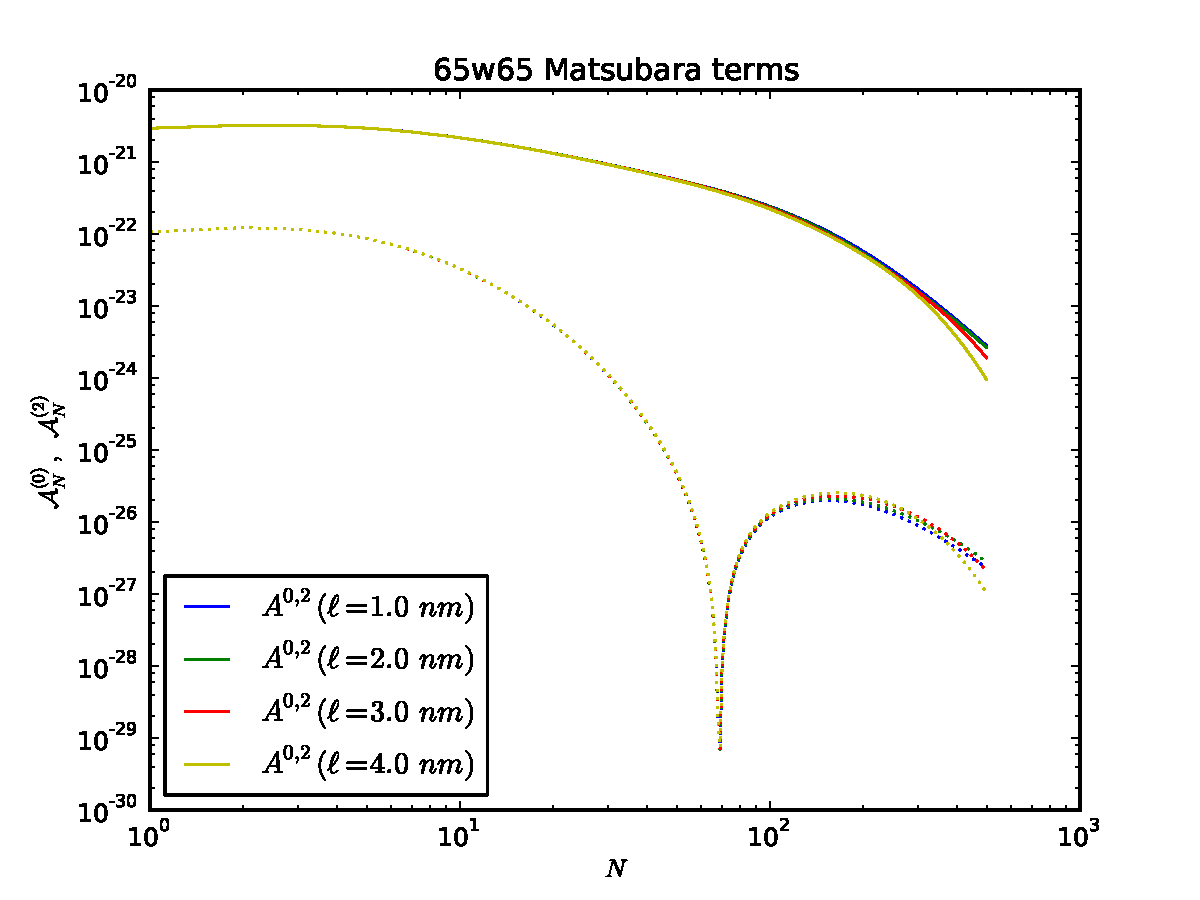
\includegraphics[width=1.2\textwidth]{plots/65_A_vs_n.pdf} (a)
\end{center}
\end{minipage}
\hskip 43pt
\begin{minipage}[b]{0.40\textwidth}
\begin{center}
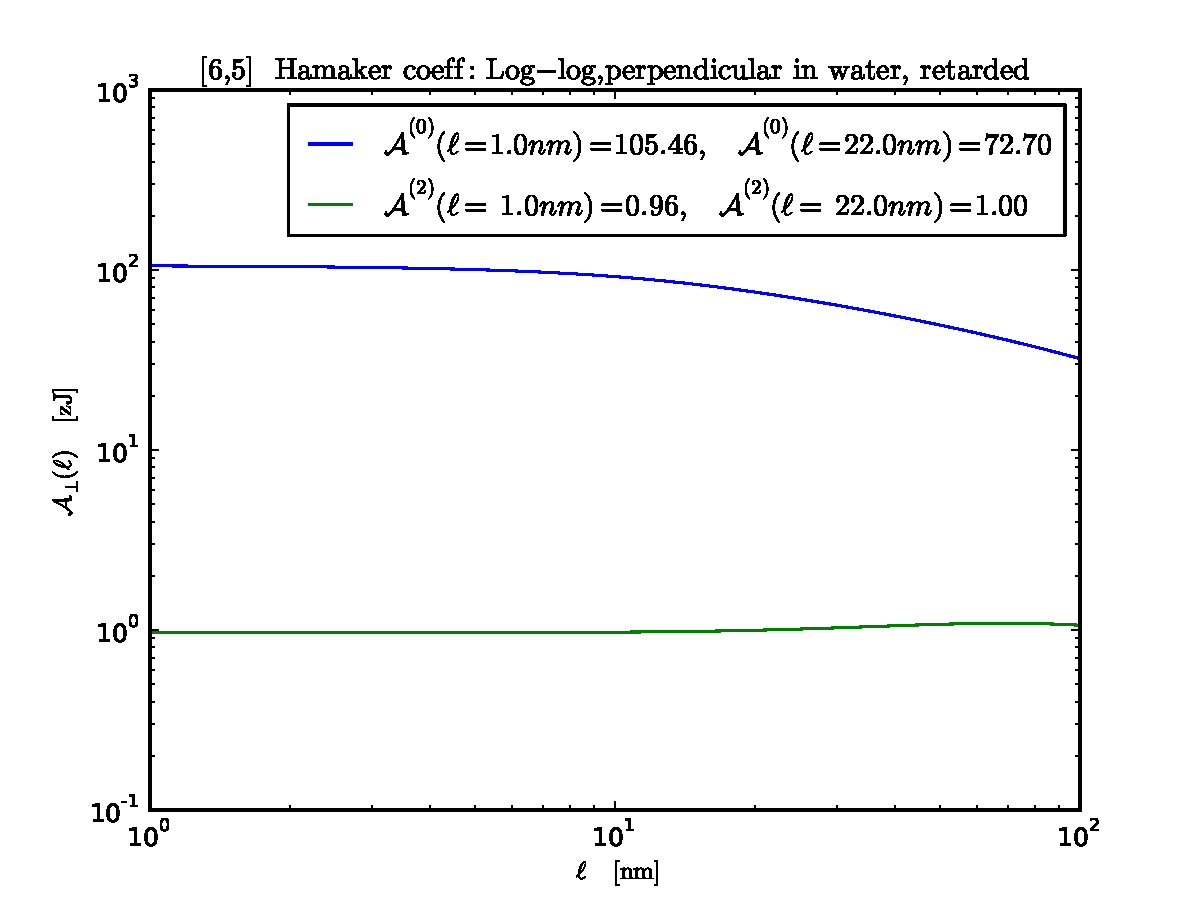
\includegraphics[width=1.2\textwidth]{plots/140322_65w65_HCs_perpendicular_ret.pdf} (b)
\end{center}
\end{minipage}
\caption{Full result using Eqs.\ref{pars-31},\ref{pars-31-g} (a) Anisotropic response functions for CG-10 DNA and water. The DNA response functions in the x and y directions were used as perpendicular and parallel inputs, respectively.  CG-10 and water eps2 data was provided by Dan Dryden. CG-10 data scales Wai-Yim's calculations by 4.94 and is assumed to include Na (more info in Dan Dryden email sent to us on Nov. 8, 2013).  Water data was built from lorentz oscillators R.H.French,J.Amer.Ceram Soc.,83,9,2117-46(2000), H.D.Ackler, et al,J.Coll.Interface Sci.179,46.
(b) Anisotropy metric $a_{1,2}(i\zeta_n)$ using Eq.\ref{eq:adef}, compares the anisotropy of the  cylinders (DNA) to their intervening material, water for the terms contruting to the Matsubara sum.}
\label{eiz65}
\end{center}
\end{figure*} 

%%%%%%%%%EPS2 and Aiz%%%%%%%%%%%%%%%%%%%%%%%%%%%%%%%%%%%%%%%%%%%%%%%%
\begin{figure*}[t!]
\begin{center}
\begin{minipage}[b]{0.40\textwidth}
\begin{center}
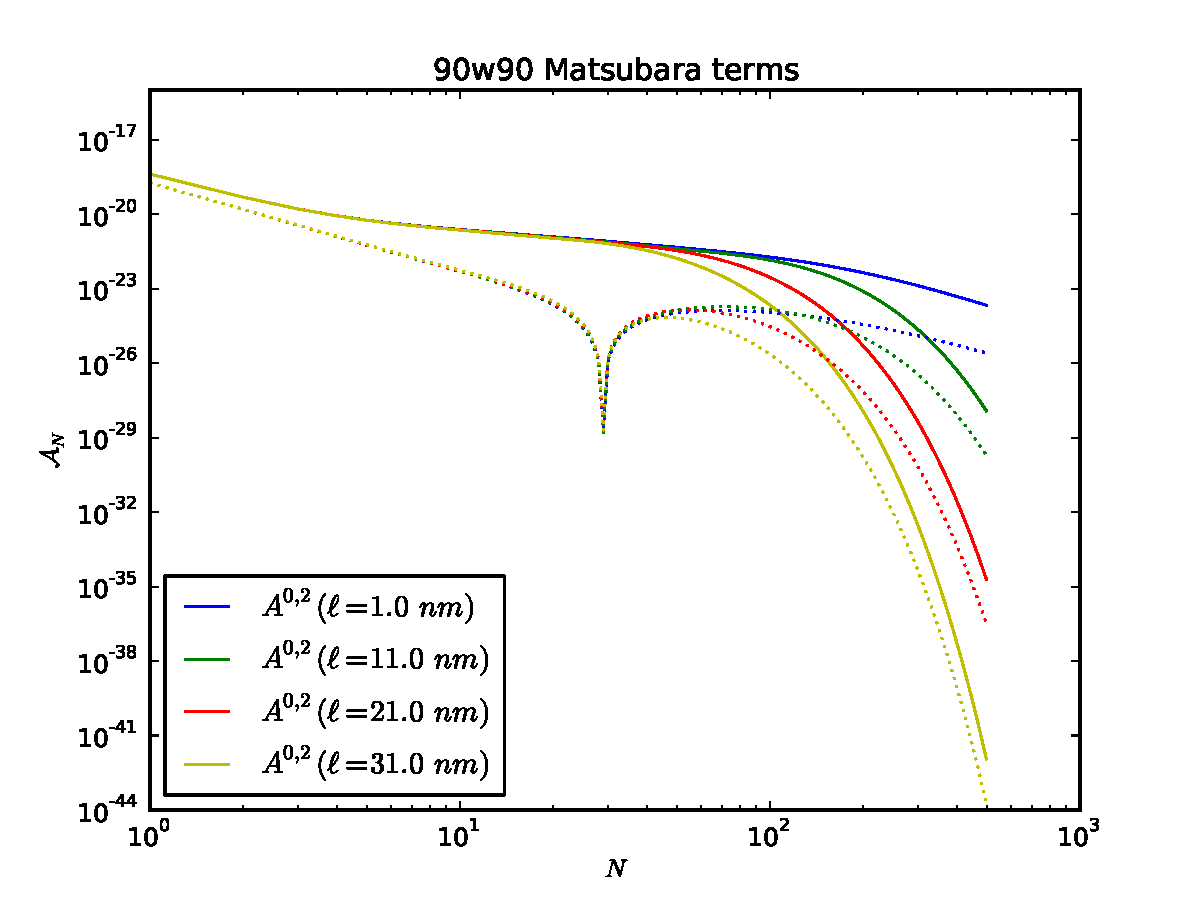
\includegraphics[width=1.2\textwidth]{plots/90_A_vs_n.pdf} (a)
\end{center}
\end{minipage}
\hskip 43pt
\begin{minipage}[b]{0.40\textwidth}
\begin{center}
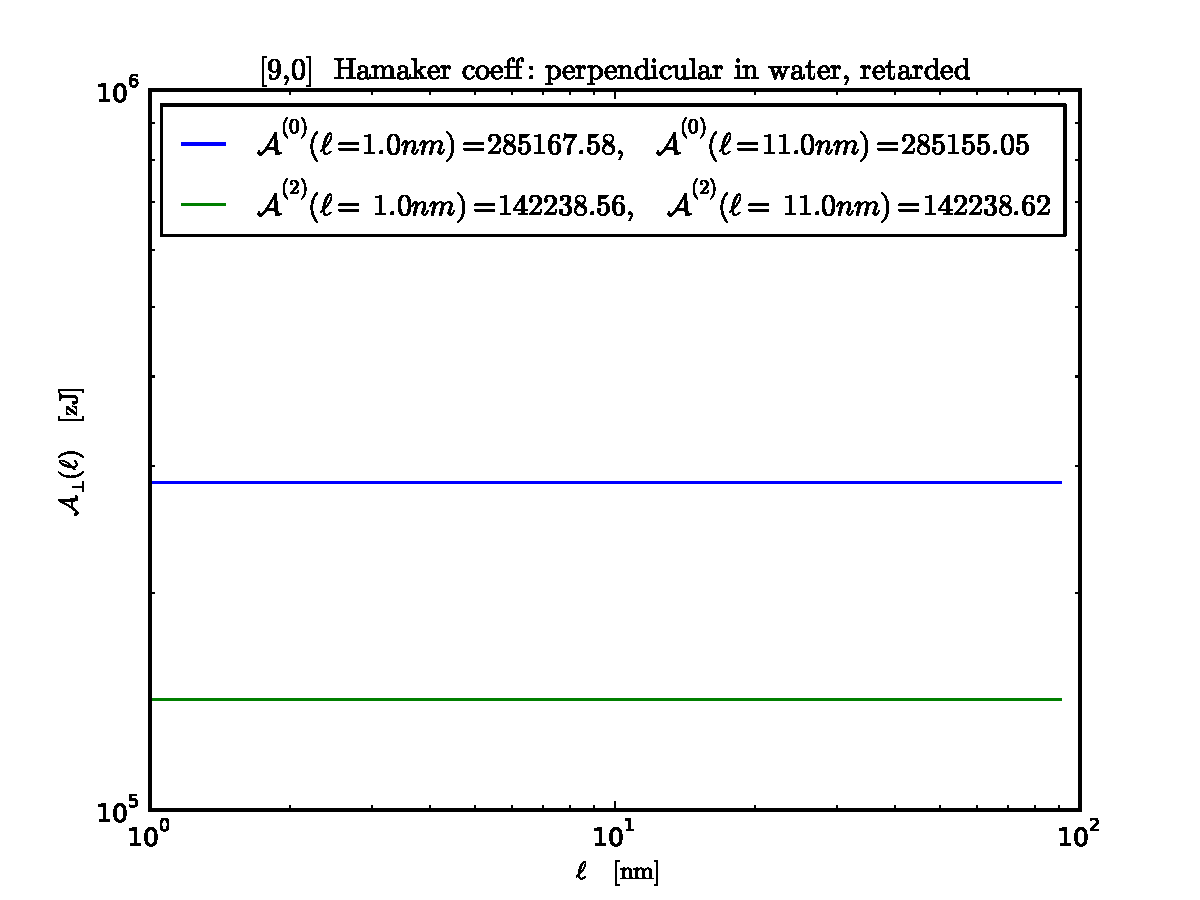
\includegraphics[width=1.2\textwidth]{plots/140322_90w90_HCs_perpendicular_ret.pdf} (b)
\end{center}
\end{minipage}
\caption{Full result using Eqs.\ref{pars-31},\ref{pars-31-g} (a) Anisotropic response functions for CG-10 DNA and water. The DNA response functions in the x and y directions were used as perpendicular and parallel inputs, respectively.  CG-10 and water eps2 data was provided by Dan Dryden. CG-10 data scales Wai-Yim's calculations by 4.94 and is assumed to include Na (more info in Dan Dryden email sent to us on Nov. 8, 2013).  Water data was built from lorentz oscillators R.H.French,J.Amer.Ceram Soc.,83,9,2117-46(2000), H.D.Ackler, et al,J.Coll.Interface Sci.179,46.
(b) Anisotropy metric $a_{1,2}(i\zeta_n)$ using Eq.\ref{eq:adef}, compares the anisotropy of the  cylinders (DNA) to their intervening material, water for the terms contruting to the Matsubara sum.}
\label{eiz65}
\end{center}
\end{figure*} 

%%%%%%%%%EPS2 and Aiz%%%%%%%%%%%%%%%%%%%%%%%%%%%%%%%%%%%%%%%%%%%%%%%%
\begin{figure*}[t!]
\begin{center}
\begin{minipage}[b]{0.40\textwidth}
\begin{center}
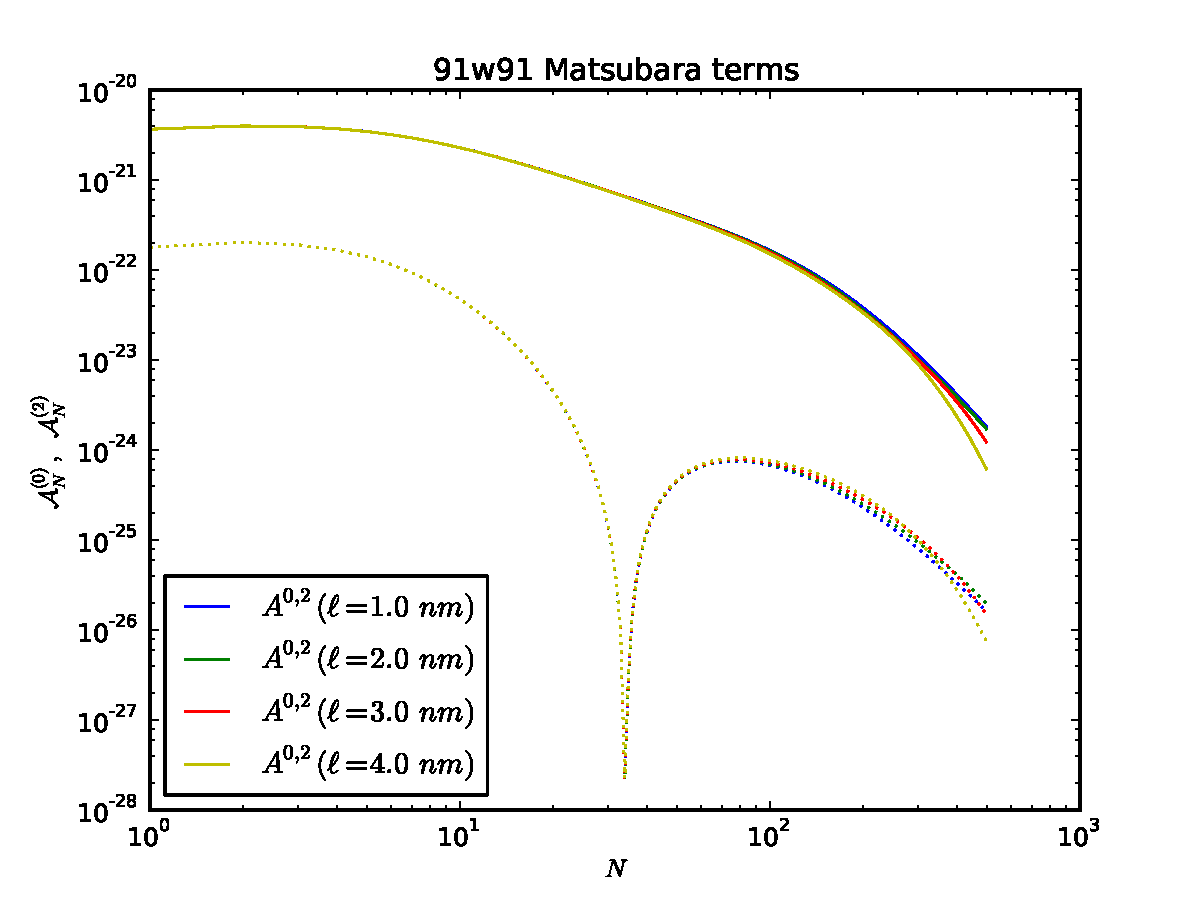
\includegraphics[width=1.2\textwidth]{plots/91_A_vs_n.pdf} (a)
\end{center}
\end{minipage}
\hskip 43pt
\begin{minipage}[b]{0.40\textwidth}
\begin{center}
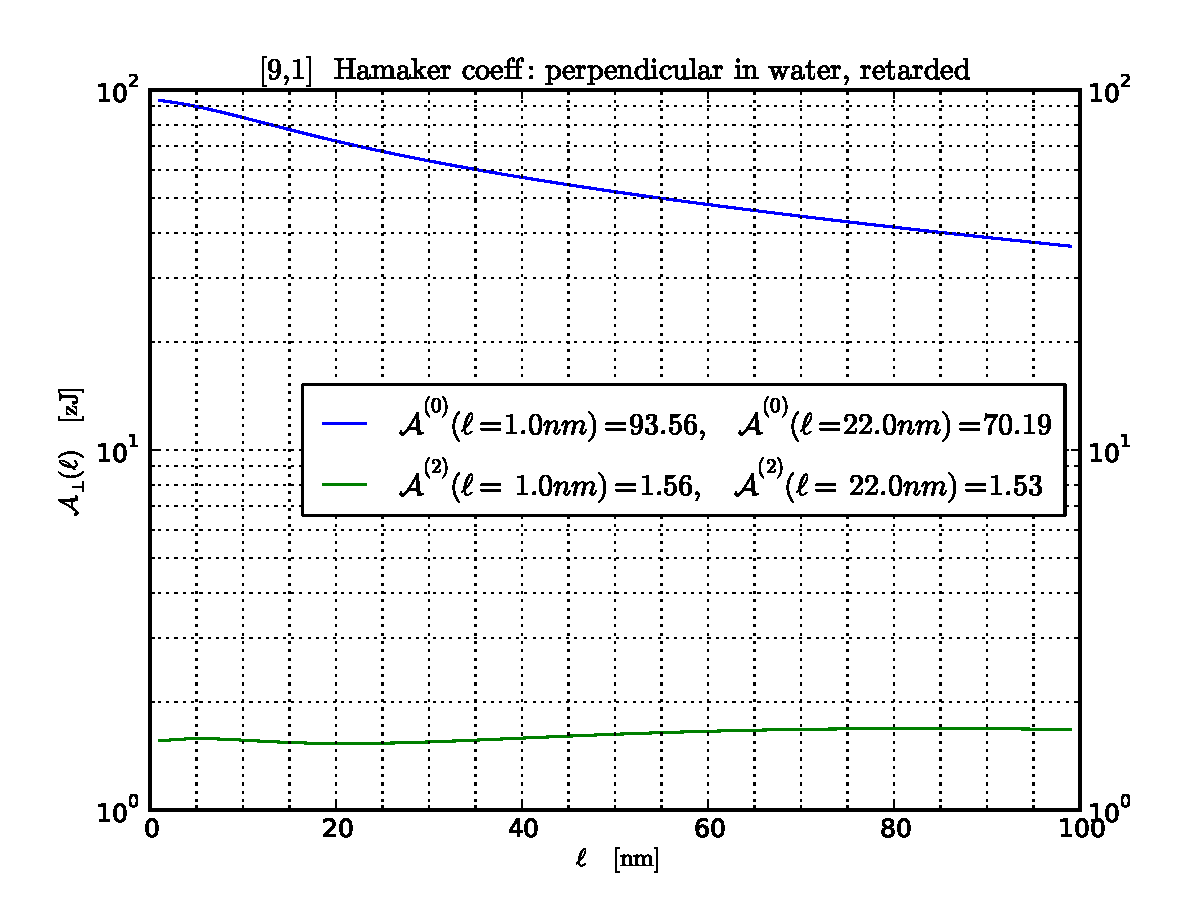
\includegraphics[width=1.2\textwidth]{plots/140322_91w91_HCs_perpendicular_ret.pdf} (b)
\end{center}
\end{minipage}
\caption{Full result using Eqs.\ref{pars-31},\ref{pars-31-g} (a) Anisotropic response functions for CG-10 DNA and water. The DNA response functions in the x and y directions were used as perpendicular and parallel inputs, respectively.  CG-10 and water eps2 data was provided by Dan Dryden. CG-10 data scales Wai-Yim's calculations by 4.94 and is assumed to include Na (more info in Dan Dryden email sent to us on Nov. 8, 2013).  Water data was built from lorentz oscillators R.H.French,J.Amer.Ceram Soc.,83,9,2117-46(2000), H.D.Ackler, et al,J.Coll.Interface Sci.179,46.
(b) Anisotropy metric $a_{1,2}(i\zeta_n)$ using Eq.\ref{eq:adef}, compares the anisotropy of the  cylinders (DNA) to their intervening material, water for the terms contruting to the Matsubara sum.}
\label{eiz65}
\end{center}
\end{figure*} 

%%%%%%%%%EPS2 and Aiz%%%%%%%%%%%%%%%%%%%%%%%%%%%%%%%%%%%%%%%%%%%%%%%%
\begin{figure*}[t!]
\begin{center}
\begin{minipage}[b]{0.40\textwidth}
\begin{center}
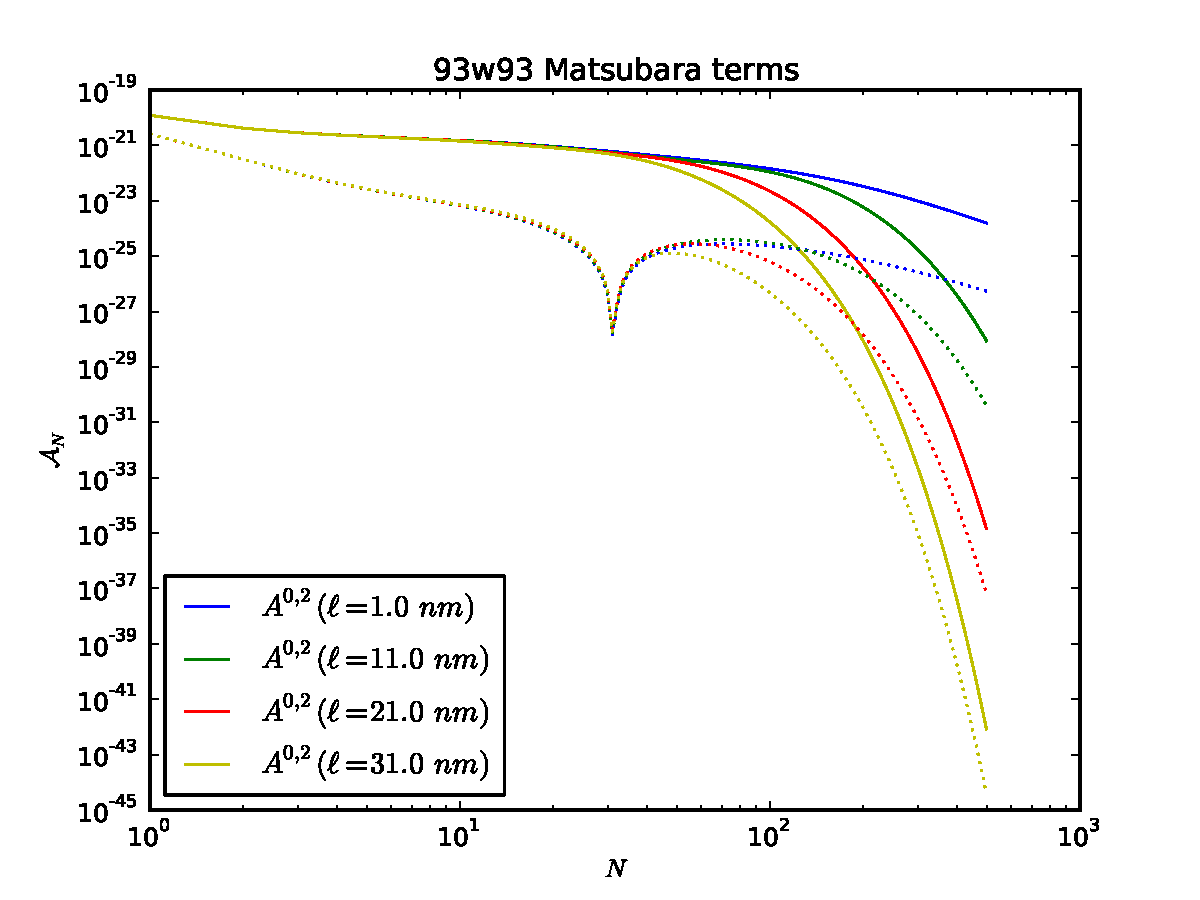
\includegraphics[width=1.2\textwidth]{plots/93_A_vs_n.pdf} (a)
\end{center}
\end{minipage}
\hskip 43pt
\begin{minipage}[b]{0.40\textwidth}
\begin{center}
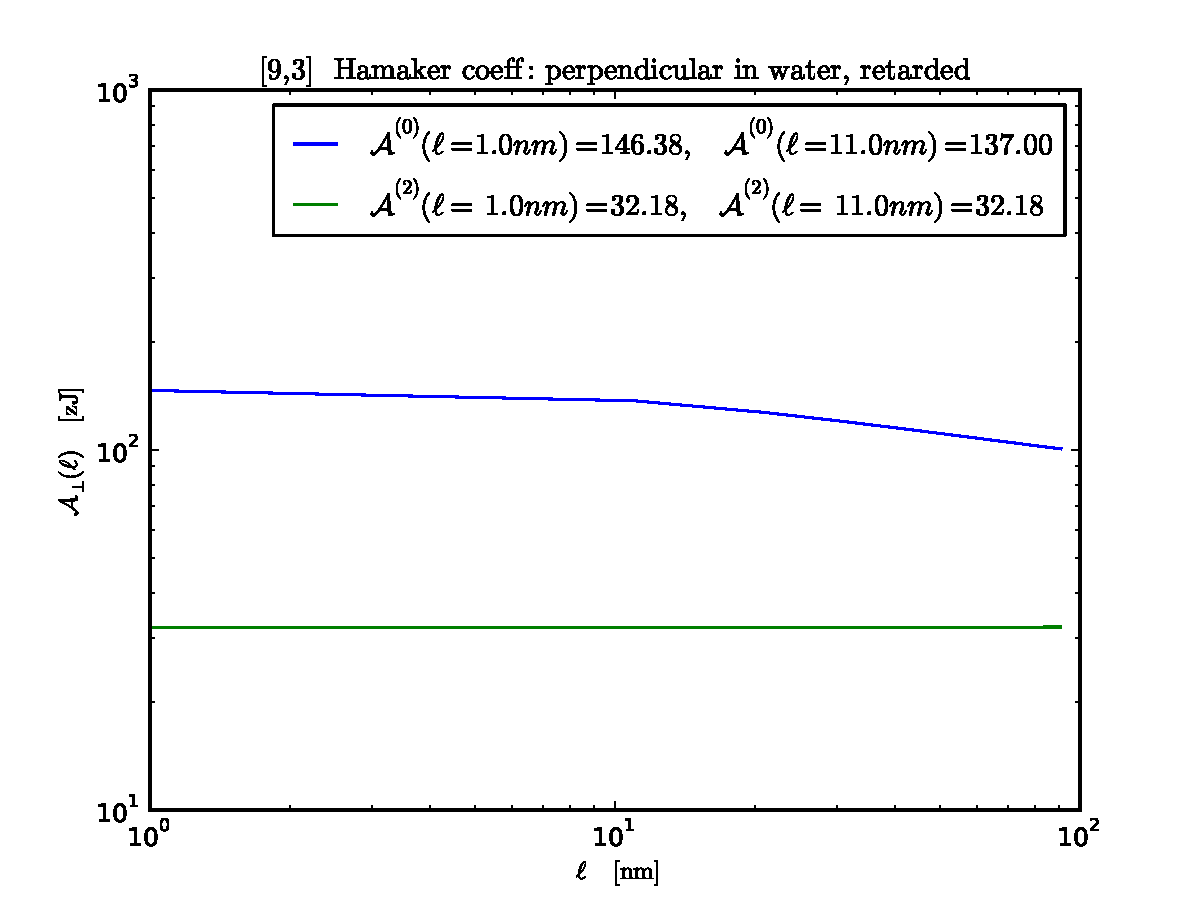
\includegraphics[width=1.2\textwidth]{plots/140322_93w93_HCs_perpendicular_ret.pdf} (b)
\end{center}
\end{minipage}
\caption{Full result using Eqs.\ref{pars-31},\ref{pars-31-g} (a) Anisotropic response functions for CG-10 DNA and water. The DNA response functions in the x and y directions were used as perpendicular and parallel inputs, respectively.  CG-10 and water eps2 data was provided by Dan Dryden. CG-10 data scales Wai-Yim's calculations by 4.94 and is assumed to include Na (more info in Dan Dryden email sent to us on Nov. 8, 2013).  Water data was built from lorentz oscillators R.H.French,J.Amer.Ceram Soc.,83,9,2117-46(2000), H.D.Ackler, et al,J.Coll.Interface Sci.179,46.
(b) Anisotropy metric $a_{1,2}(i\zeta_n)$ using Eq.\ref{eq:adef}, compares the anisotropy of the  cylinders (DNA) to their intervening material, water for the terms contruting to the Matsubara sum.}
\label{eiz65}
\end{center}
\end{figure*} 

%%%%%%%%%EPS2 and Aiz%%%%%%%%%%%%%%%%%%%%%%%%%%%%%%%%%%%%%%%%%%%%%%%%
\begin{figure*}[t!]
\begin{center}
\begin{minipage}[b]{0.40\textwidth}
\begin{center}
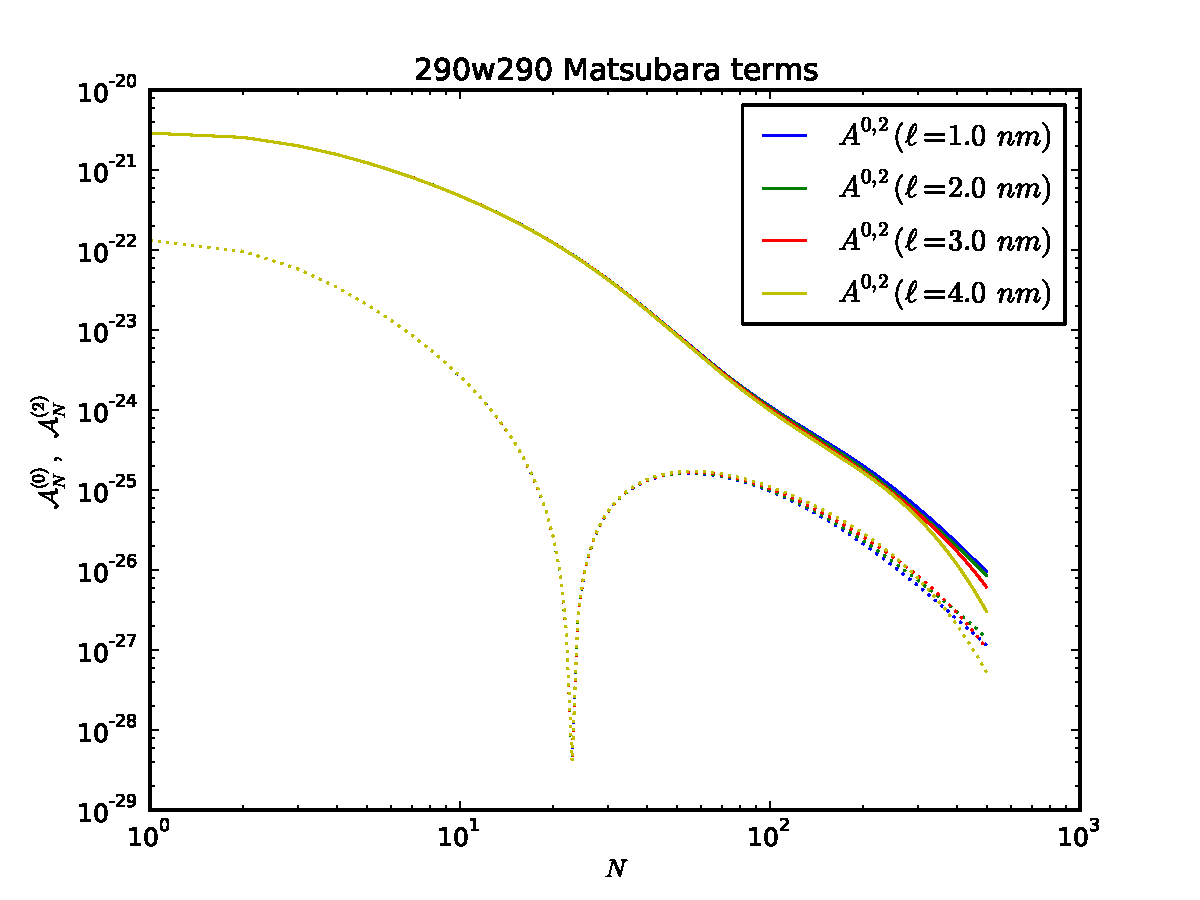
\includegraphics[width=1.2\textwidth]{plots/290_A_vs_n.pdf} (a)
\end{center}
\end{minipage}
\hskip 43pt
\begin{minipage}[b]{0.40\textwidth}
\begin{center}
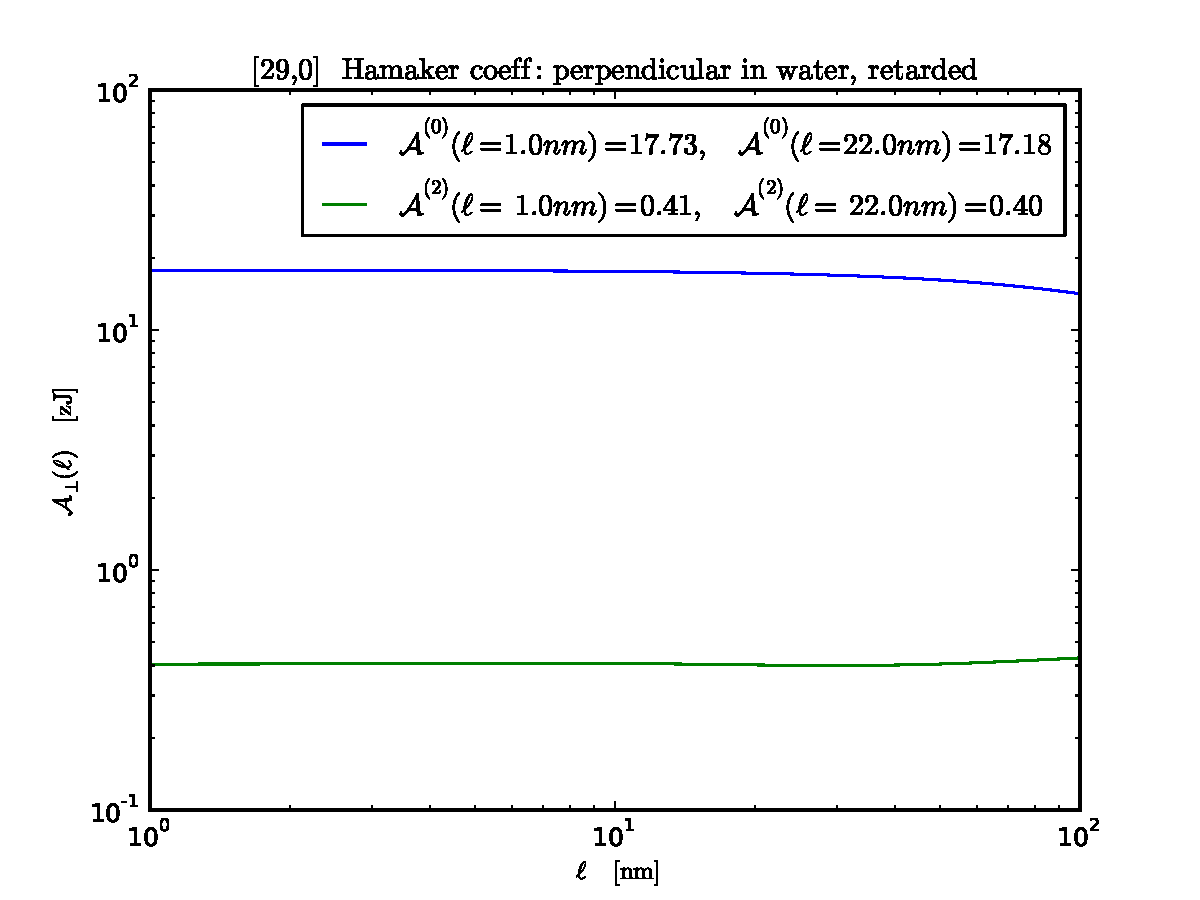
\includegraphics[width=1.2\textwidth]{plots/140322_290w290_HCs_perpendicular_ret.pdf} (b)
\end{center}
\end{minipage}
\caption{Full result using Eqs.\ref{pars-31},\ref{pars-31-g} (a) Anisotropic response functions for CG-10 DNA and water. The DNA response functions in the x and y directions were used as perpendicular and parallel inputs, respectively.  CG-10 and water eps2 data was provided by Dan Dryden. CG-10 data scales Wai-Yim's calculations by 4.94 and is assumed to include Na (more info in Dan Dryden email sent to us on Nov. 8, 2013).  Water data was built from lorentz oscillators R.H.French,J.Amer.Ceram Soc.,83,9,2117-46(2000), H.D.Ackler, et al,J.Coll.Interface Sci.179,46.
(b) Anisotropy metric $a_{1,2}(i\zeta_n)$ using Eq.\ref{eq:adef}, compares the anisotropy of the  cylinders (DNA) to their intervening material, water for the terms contruting to the Matsubara sum.}
\label{eiz65}
\end{center}
\end{figure*} 

\begin{figure}
\centerline{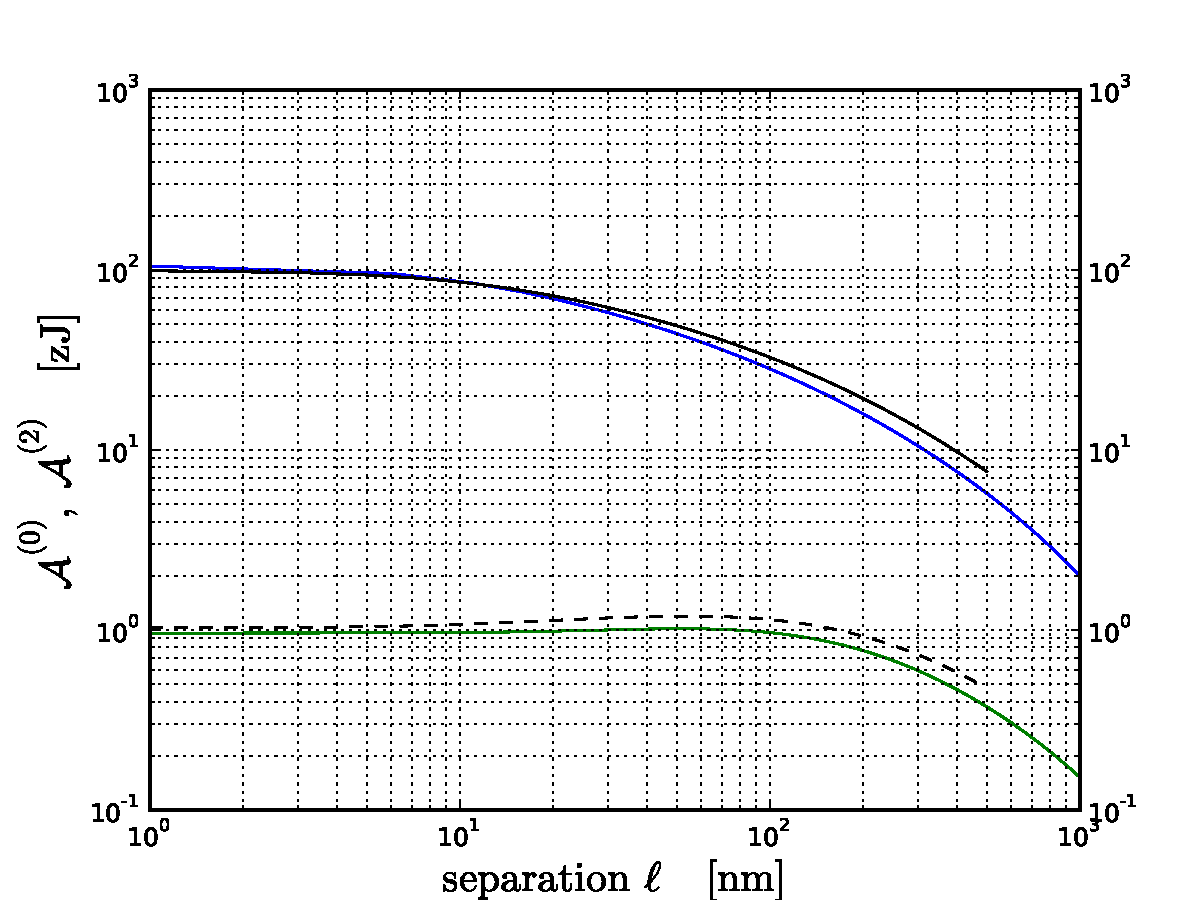
\includegraphics[width=12cm]{140309_65w65_GH_skew_ret_A0_A2.pdf}}
%\epsfig {file=sketch.pdf,width=5cm}}
\caption{A sketch of the system of interest (the two cylinders). The quantities describing the geometry of the system are 
denoted, together with the logitudinal and transverse directions of cylinder in the left half-space (1). The skew angle $\theta$ is about an axis normal to the planar boundary defining the limits of each half-space.
}
\label{fig:sketch}
\end{figure}

\begin{figure}
\centerline{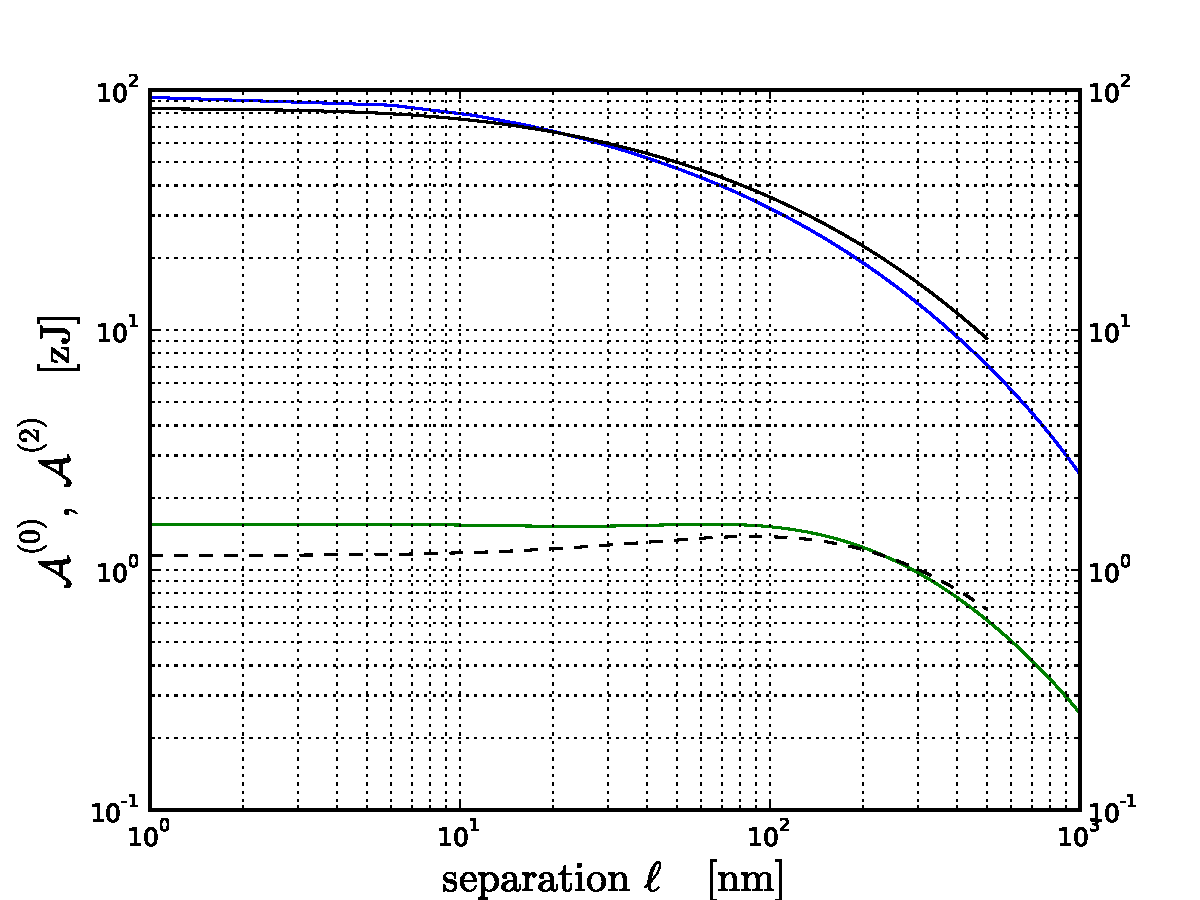
\includegraphics[width= 12cm]{140309_91w91_GH_skew_ret_A0_A2.pdf}}
%\epsfig {file=sketch.pdf,width=5cm}}
\caption{A sketch of the system of interest (the two cylinders). The quantities describing the geometry of the system are 
denoted, together with the logitudinal and transverse directions of cylinder in the left half-space (1). The skew angle $\theta$ is about an axis normal to the planar boundary defining the limits of each half-space.
}
\label{fig:sketch}
\end{figure}

\begin{figure}
\centerline{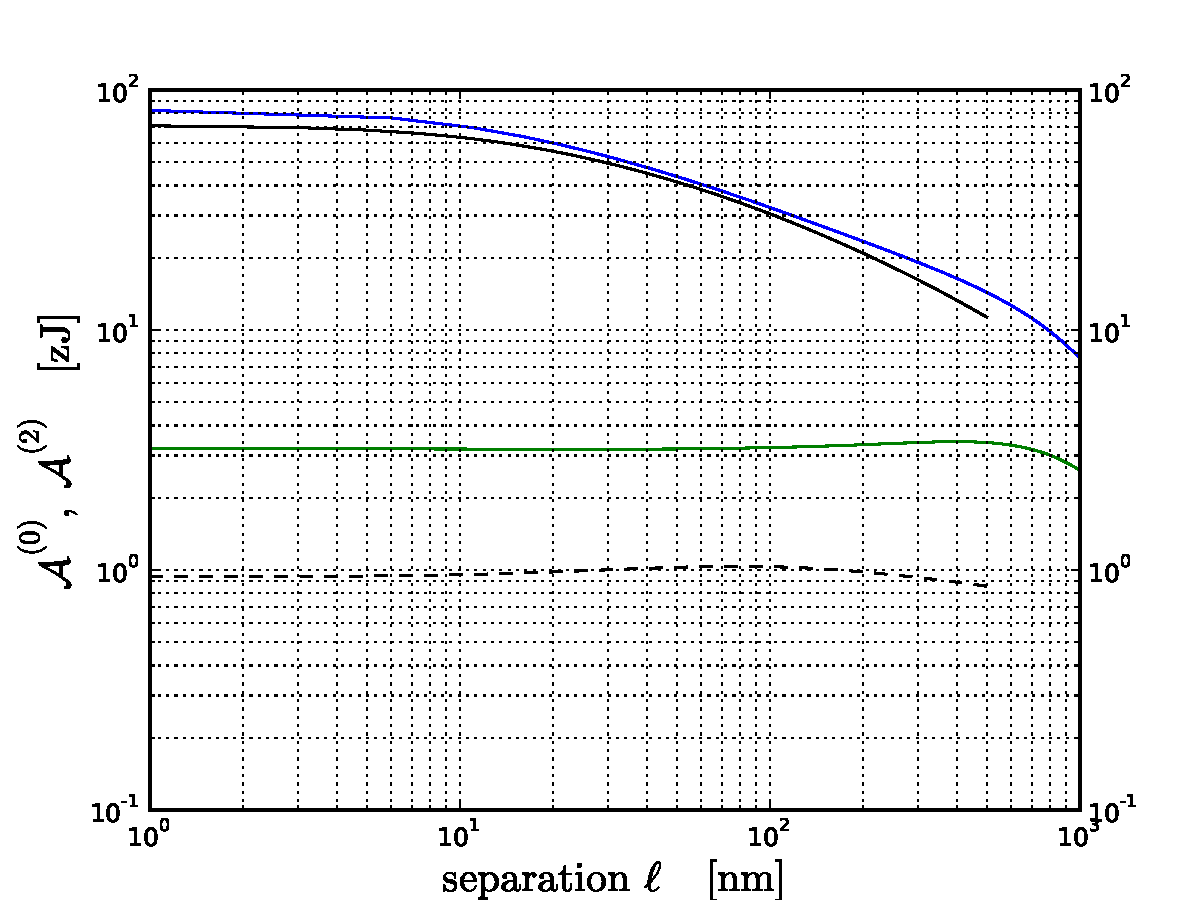
\includegraphics[width=12cm]{140309_93w93_GH_skew_ret_A0_A2.pdf}}
%\epsfig {file=sketch.pdf,width=5cm}}
\caption{A sketch of the system of interest (the two cylinders). The quantities describing the geometry of the system are 
denoted, together with the logitudinal and transverse directions of cylinder in the left half-space (1). The skew angle $\theta$ is about an axis normal to the planar boundary defining the limits of each half-space.
}
\label{fig:sketch}
\end{figure}

\begin{figure}
\centerline{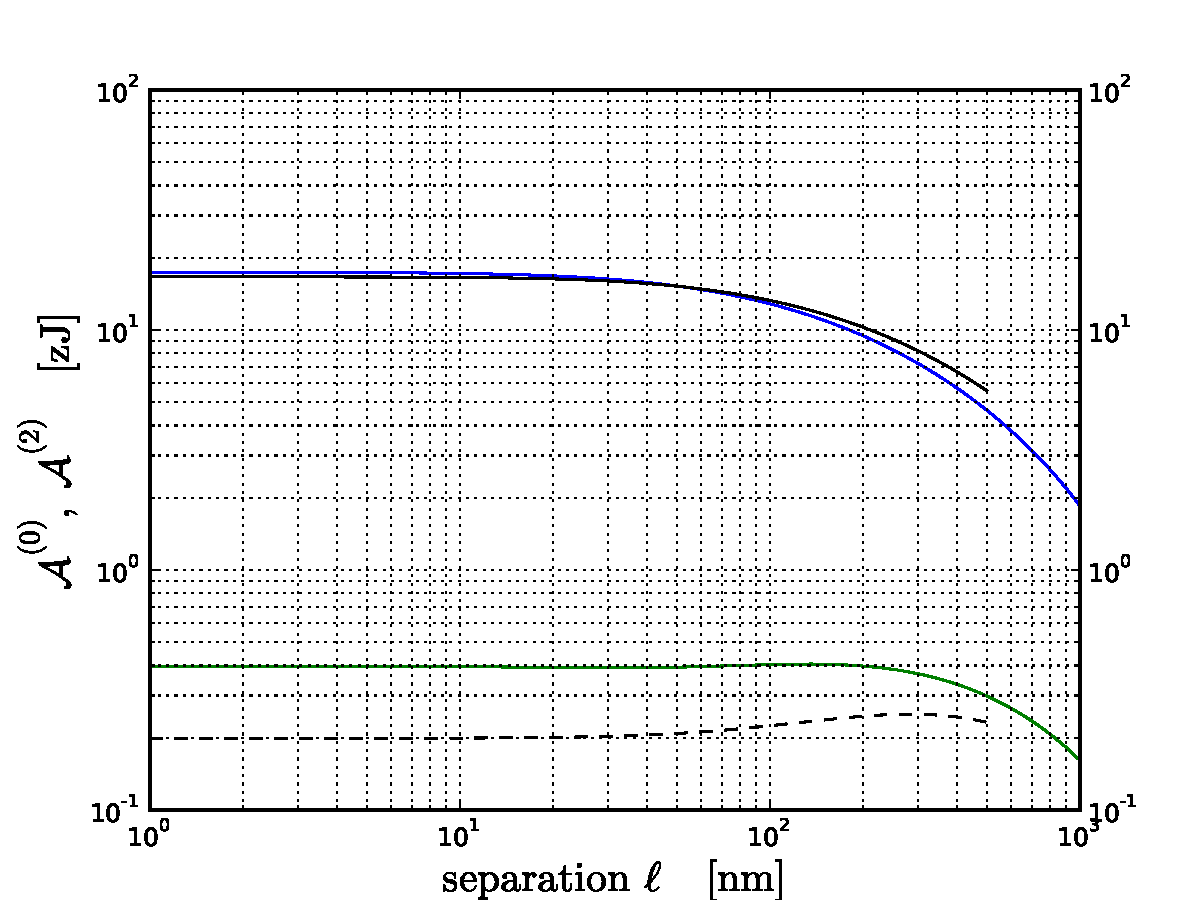
\includegraphics[width=12cm]{140309_290w290_GH_skew_ret_A0_A2.pdf}}
%\epsfig {file=sketch.pdf,width=5cm}}
\caption{A sketch of the system of interest (the two cylinders). The quantities describing the geometry of the system are 
denoted, together with the logitudinal and transverse directions of cylinder in the left half-space (1). The skew angle $\theta$ is about an axis normal to the planar boundary defining the limits of each half-space.
}
\label{fig:sketch}
\end{figure}

We use  Eq. \ref{form1} to obtain the interaction free energy between two skewed cylinders:
\begin{equation}
G(\ell,\theta) = - \frac{k_BT}{64 \pi} \frac{ \pi^2 R_1^{2} R_2^{2} }{\ell^{4} \sin{\theta}} {\sum_{n=0}^{\infty}}' \Delta_{1,\parallel} \Delta_{2,\parallel} \int_0^{\infty}  u du ~\frac{e^{- 2 \sqrt{u^{2} + p_n^{2}}}}{(u^{2} + p_n^{2})}  g(a_1, a_2, u, p_n, \theta),
\label{pars-3}
\end{equation}
where $u = Q \ell$,  
\begin{widetext}
\begin{eqnarray}
g(a_1, a_2, u, p_n, \theta) &=&  2 \left[ (1+3a_1)(1+3a_2) u^{4} + 2(1+2a_1+2a_2+3a_1a_2) u^{2}p_n^{2}  + 2(1+a_1)(1+a_2) p_n^{4}\right] + \nonumber \\ 
& & ~~~~~~~~~~~~~~~~~~~~~~~~~~~~~~~~~~~~~~~~~ + (1-a_1)(1-a_2)(u^{2} + 2 p_n^{2})^2 \cos 2\theta
\end{eqnarray}
\end{widetext}
and $p_n^{2}(\ell) =  \epsilon_m(i \omega_n) \frac{\omega_n^{2}}{c^{2}} \ell^{2}$. Another change of variables with $u = p_n t$, yields 
\begin{equation}
G(\ell,\theta) = - \frac{k_BT}{64 \pi} \frac{ \pi^2 R_1^{2} R_2^{2} }{\ell^{4} \sin{\theta}} {\sum_{n=0}^{\infty}}' \Delta_{1,\parallel} \Delta_{2,\parallel} ~p_n^{4} ~\int_0^{\infty} t dt ~\frac{e^{- 2 p_n \sqrt{t^{2} + 1}}}{(t^{2} + 1)} \tilde g(t, a_1(i \omega_n), a_2(i \omega_n), \theta),
\label{pars-31}
\end{equation}
with
\begin{widetext}
\begin{eqnarray}
\tilde g(t, a_1, a_2, \theta) &=& 2 \left[ (1+3a_1)(1+3a_2) t^{4} + 2 (1+2a_1+2a_2+3a_1a_2) t^{2}  + 2(1+a_1)(1+a_2)\right] + \nonumber \\
& & ~~~~~~~~~~~~~~~~~~~~~~~~~~~~~~~~~~~~~~~~~ + (1-a_1)(1-a_2)(t^{2} + 2)^2 \cos 2\theta.
\label{pars-31-g}
\end{eqnarray}
\end{widetext}
The cylinder-cylinder interaction at all angles when the radii of the cylinders are the smallest lengths in the system. It includes retardation and the full angular dependence:
\begin{equation}
  \fbox{
    $\displaystyle{
G(\ell,\theta) = - \frac{ (\pi R_1^{2})(\pi R_2^{2}) }{2 \pi~\ell^{4} \sin{\theta}} \left( {\cal A}^{(0)}(\ell) + {\cal A}^{(2)}(\ell) \cos 2\theta \right) ,}$}
\label{pars-31a}
\end{equation}
Where $(\ell)$  is the inter surface separation. The $(\ell)$ dependence of the Hamaker coefficients $\cal A$ is a consequence of $(\ell)$ dependence of $p_n^{2}(\ell) =  \epsilon_m(i \omega_n) \frac{\omega_n^{2}}{c^{2}} \ell^{2}$. Above we defined
\begin{widetext}
\begin{equation}
{\cal A}^{(0)}(\ell) = \frac{k_BT}{32}  {\sum_{n=0}^{\infty}}' \Delta_{1,\parallel} \Delta_{2,\parallel} ~p_n^{4}(\ell) ~\int_0^{\infty} t dt ~\frac{e^{- 2 p_n(\ell) \sqrt{t^{2} + 1}}}{(t^{2} + 1)} \tilde g^{(0)}(t, a_1(i \omega_n), a_2(i \omega_n))
\label{eq:a0}
\end{equation}
\end{widetext}
with
\begin{equation}
\tilde g^{(0)}(t, a_1(i \omega_n), a_2(i \omega_n)) = 2 \left[ (1+3a_1)(1+3a_2) t^{4} + 2 (1+2a_1+2a_2+3a_1a_2) t^{2}  + 2(1+a_1)(1+a_2)\right]
\end{equation}
and
\begin{widetext}
\begin{equation}
{\cal A}^{(2)}(\ell) = \frac{k_BT}{32}  {\sum_{n=0}^{\infty}}' \Delta_{1,\parallel} \Delta_{2,\parallel} ~p_n^{4}(\ell) ~\int_0^{\infty} t dt ~\frac{e^{- 2 p_n(\ell) \sqrt{t^{2} + 1}}}{(t^{2} + 1)} \tilde g^{(2)}(t, a_1(i \omega_n), a_2(i \omega_n), \theta)
\end{equation}
\end{widetext}
with
\begin{equation}<C-LeftRelease>
\tilde g^{(2)}(t, a_1(i \omega_n), a_2(i \omega_n), \theta) = (1-a_1)(1-a_2)(t^{2} + 2)^2
\label{befgqw}
\end{equation}

The numerical implementation should be for Eqs. \ref{pars-31a}-\ref{befgqw}. For $a_{1,2}$ one invokes the previous definition Eq. \ref{eq:adef}
\begin{equation}
a_{1,2}(i \omega_n) = \frac{2 \Delta_{\perp}^{(1,2)}(i \omega_n)}{\Delta_{\parallel}^{(1,2)}(i \omega_n)} = 2 \frac{({{\epsilon^{c}}_{\perp}}^{(1,2)}(i \omega_n) -\epsilon_{m}(i \omega_n)) \epsilon_{m}(i \omega_n)}{({{\epsilon^{c}}_{\perp}}^{(1,2)}(i \omega_n)+\epsilon_{m}(i \omega_n)) ({{\epsilon^{c}}_{\parallel}}^{(1,2)}(i \omega_n) -\epsilon_{m}(i \omega_n))}
\label{eq:adef}
\end{equation}
where ${{\epsilon^{c}}_{\perp}}^{(1,2)}$, ${{\epsilon^{c}}_{\parallel}}^{(1,2)}$ are the perpendicular, parallel components of the dielectric response functions of the two cylinders and $\epsilon_{m}$ is the same for the medium in between. All these quantities are of course frequency dependent. The $n$ summation is over the Matsubara frequencies, $\zeta_n = 2\pi n k_BT/\hbar$, where $n$ is an integer and the $n=0$ term is counted with a weight $1/2$. At room temperature the Matsubara frequencies are a multiple of $\rm 2.4 \times 10^{14}~s^{-1}$.

\begin{table}[ht]
\caption{Hamaker coefficents for perpendiuclar, retarded formulation at
intersurface distance of 1 nm}% title of Table
\centering
% used for centering table
\begin{tabular}{c c c c}
% centered columns (4 columns)
\hline\hline
%inserts double horizontal lines
Case & Method\#1 & Method\#2 & Method\#3 \\ [0.5ex]
% inserts table
%heading
\hline
% inserts single horizontal line
1 & 50 & 837 & 970 \\
% inserting body of the table
2 & 47 & 877 & 230 \\
3 & 31 & 25 & 415 \\
4 & 35 & 144 & 2356 \\
5 & 45 & 300 & 556 \\ [1ex]
% [1ex] adds vertical space
\hline
%inserts single line
\end{tabular}
\label{table:nonlin}
% is used to refer this table in the text

\end{table}

\begin{table}[ht]
\caption{Hamaker coefficents, retarded formulation: perpendiuclar cylinders
in water, intersurface distance = 1 nm}% title of Table
\centering
% used for centering table
\begin{tabular}{l c|c|c}
  \hline  
  &\hspace{0.25in}CNT \hspace{0.25in}& \hspace{0.25in}$\mathcal{A}^{0}$    [zJ] \hspace{0.25in}& \hspace{0.25in}$\mathcal{A}^{2}$    [zJ] \hspace{0.25in}\\
  \hline\hline 
  &[6,5]  & 105.46 & 0.96 \\
  \hline
  &[9,0]  & \multicolumn{2}{c}{semi-metal; in progress}\\
  \hline
  &[9,1]  & 93.56 & 1.56 \\
  \hline
  &[9,0]  & \multicolumn{2}{c}{semi-metal; in progress}\\
  \hline
  &[29,0] & 17.73 & 0.41 \\
  \hline  
\end{tabular}
\label{table:nonlin}
% is used to refer this table in the text

\end{table}

\begin{table}[ht]
\caption{Hamaker coefficents, non-retarded formulation: perpendiuclar cylinders in water}% title of Table
\centering
% used for centering table
\begin{tabular}{r c | c | c}
  \hline
  &\hspace{0.25in}CNT \hspace{0.25in}& \hspace{0.25in}$\mathcal{A}^{0}$    [zJ] \hspace{0.25in}& \hspace{0.25in}$\mathcal{A}^{2}$    [zJ] \hspace{0.25in}\\
  \hline\hline                       
  &[6,5]  & 126.80 & 1.16 \\
  \hline
  &[9,0]  & \multicolumn{2}{c}{semi-metal; in progress}\\
  \hline
  &[9,1]  & 112.22 & 1.87 \\
  \hline
  &[9,3]  & \multicolumn{2}{c}{semi-metal; in progress}\\
  \hline
  &[29,0] & 20.93 & 0.49 \\
  \hline  
\end{tabular}
\label{table:nonlin}
% is used to refer this table in the text

\end{table}

\section{Parallel cylinders}

The interaction free energy {\sl per unit length}, $g(\ell)$, between two parallel cylinders is given by the Abel transform (see e.g. Ref. \onlinecite{Parsegian}, pp 233-235)
\begin{equation}
\frac{d^{2}{\cal G}(\ell,\theta=0)}{d\ell^{2}}=N_1 N_2\int_{-\infty}^{+\infty}g(\sqrt{\ell^{2}+y^{2}})~dy.
\label{form2}
\end{equation}

\subsection{Fully retarded}

As before, we introduce $p_n^{2} =  \epsilon_m(i \omega_n) \frac{\omega_n^{2}}{c^{2}} \ell^{2}$, $u = Q\ell$ and $y \longrightarrow y/\ell$. This allows us to rewrite the above integrals as
\begin{widetext}
\begin{equation}
g(\ell) = - \frac{k_BT}{32} \frac{R_1^{2} R_2^{2}}{\ell^5} {\sum_{n=0}^{\infty}}' \Delta_{1,\parallel} \Delta_{2,\parallel} 
\int_{1}^{+\infty}\!\!\!\!\! \frac{dy}{\sqrt{y^2 - 1}} \int_0^{\infty}\!\!\!  u du ~\frac{e^{-2 y \sqrt{u^{2} + p_n^{2}}}}{(u^{2} +p_n^{2})^{1/2}} ~h(a_1(i \omega_n), a_2(i \omega_n), u, p_n^{2}),
\label{retardedfinal}
\end{equation}
\end{widetext}
and
\begin{widetext}
\begin{eqnarray}
h(a_1(i \omega_n), a_2(i \omega_n), u, p_n^{2}) &=&   2 \left[ (1+3a_1)(1+3a_2) u^{4} + 2 (1+2a_1+2a_2+3a_1a_2) u^{2} p_n^{2} + 2(1+a_1)(1+a_2) p_n^{4}\right]  + \nonumber \\
& &  (1-a_1) (1-a_2) (u^{2} + 2 p_n^{2})^2 .
\label{fcfenhjqwk}
\end{eqnarray}
\end{widetext}

We now again transform this result into a form that is suitable for computation and numerical implementation. Rewriting Eq. \ref{retardedfinal} as
\begin{equation}
  \fbox{
    $\displaystyle{
g(\ell) = - \frac{3 (\pi R_1^{2}) (\pi R_2^{2})}{8\pi~\ell^5} {\cal A}(\ell),}$}
\label{retardedfinal-a}
\end{equation}
we introduced the Hamaker coefficient
\begin{equation}
{\cal A}(\ell) = \frac{k_BT}{12 \pi} {\sum_{n=0}^{\infty}}' \Delta_{1,\parallel} \Delta_{2,\parallel} 
\int_{1}^{+\infty}\!\!\!\!\! \frac{dy}{\sqrt{y^2 - 1}} \int_0^{\infty}\!\!\!  u du ~\frac{e^{-2 y \sqrt{u^{2} + p_n^{2}(\ell)}}}{(u^{2} +p_n^{2}(\ell))^{1/2}} ~h(a_1(i \omega_n), a_2(i \omega_n), u, p_n^{2}(\ell))
\label{retardedfinal-b}
\end{equation}
with $h(a_1(i \omega_n), a_2(i \omega_n), u, p_n^{2}(\ell))$ defined in Eq. \ref{fcfenhjqwk}. This result is simpler then in the skewed case becasue it does not contain any angle dependence. In general ${\cal A}(\ell)$ can not be written in terms of ${\cal A}^{(0)}(\ell)$ and ${\cal A}^{(2)}(\ell)$ of the skewed cylinders.

%%%%%%%%%%%%%%%%%%%%%%%%%%%%%%%%%%%%%%%%%%%%%%%%%%%%%%%%%%%%%%%%%%%%%%%%%%%%%%%
%Par_ret
\begin{figure}
    \centerline{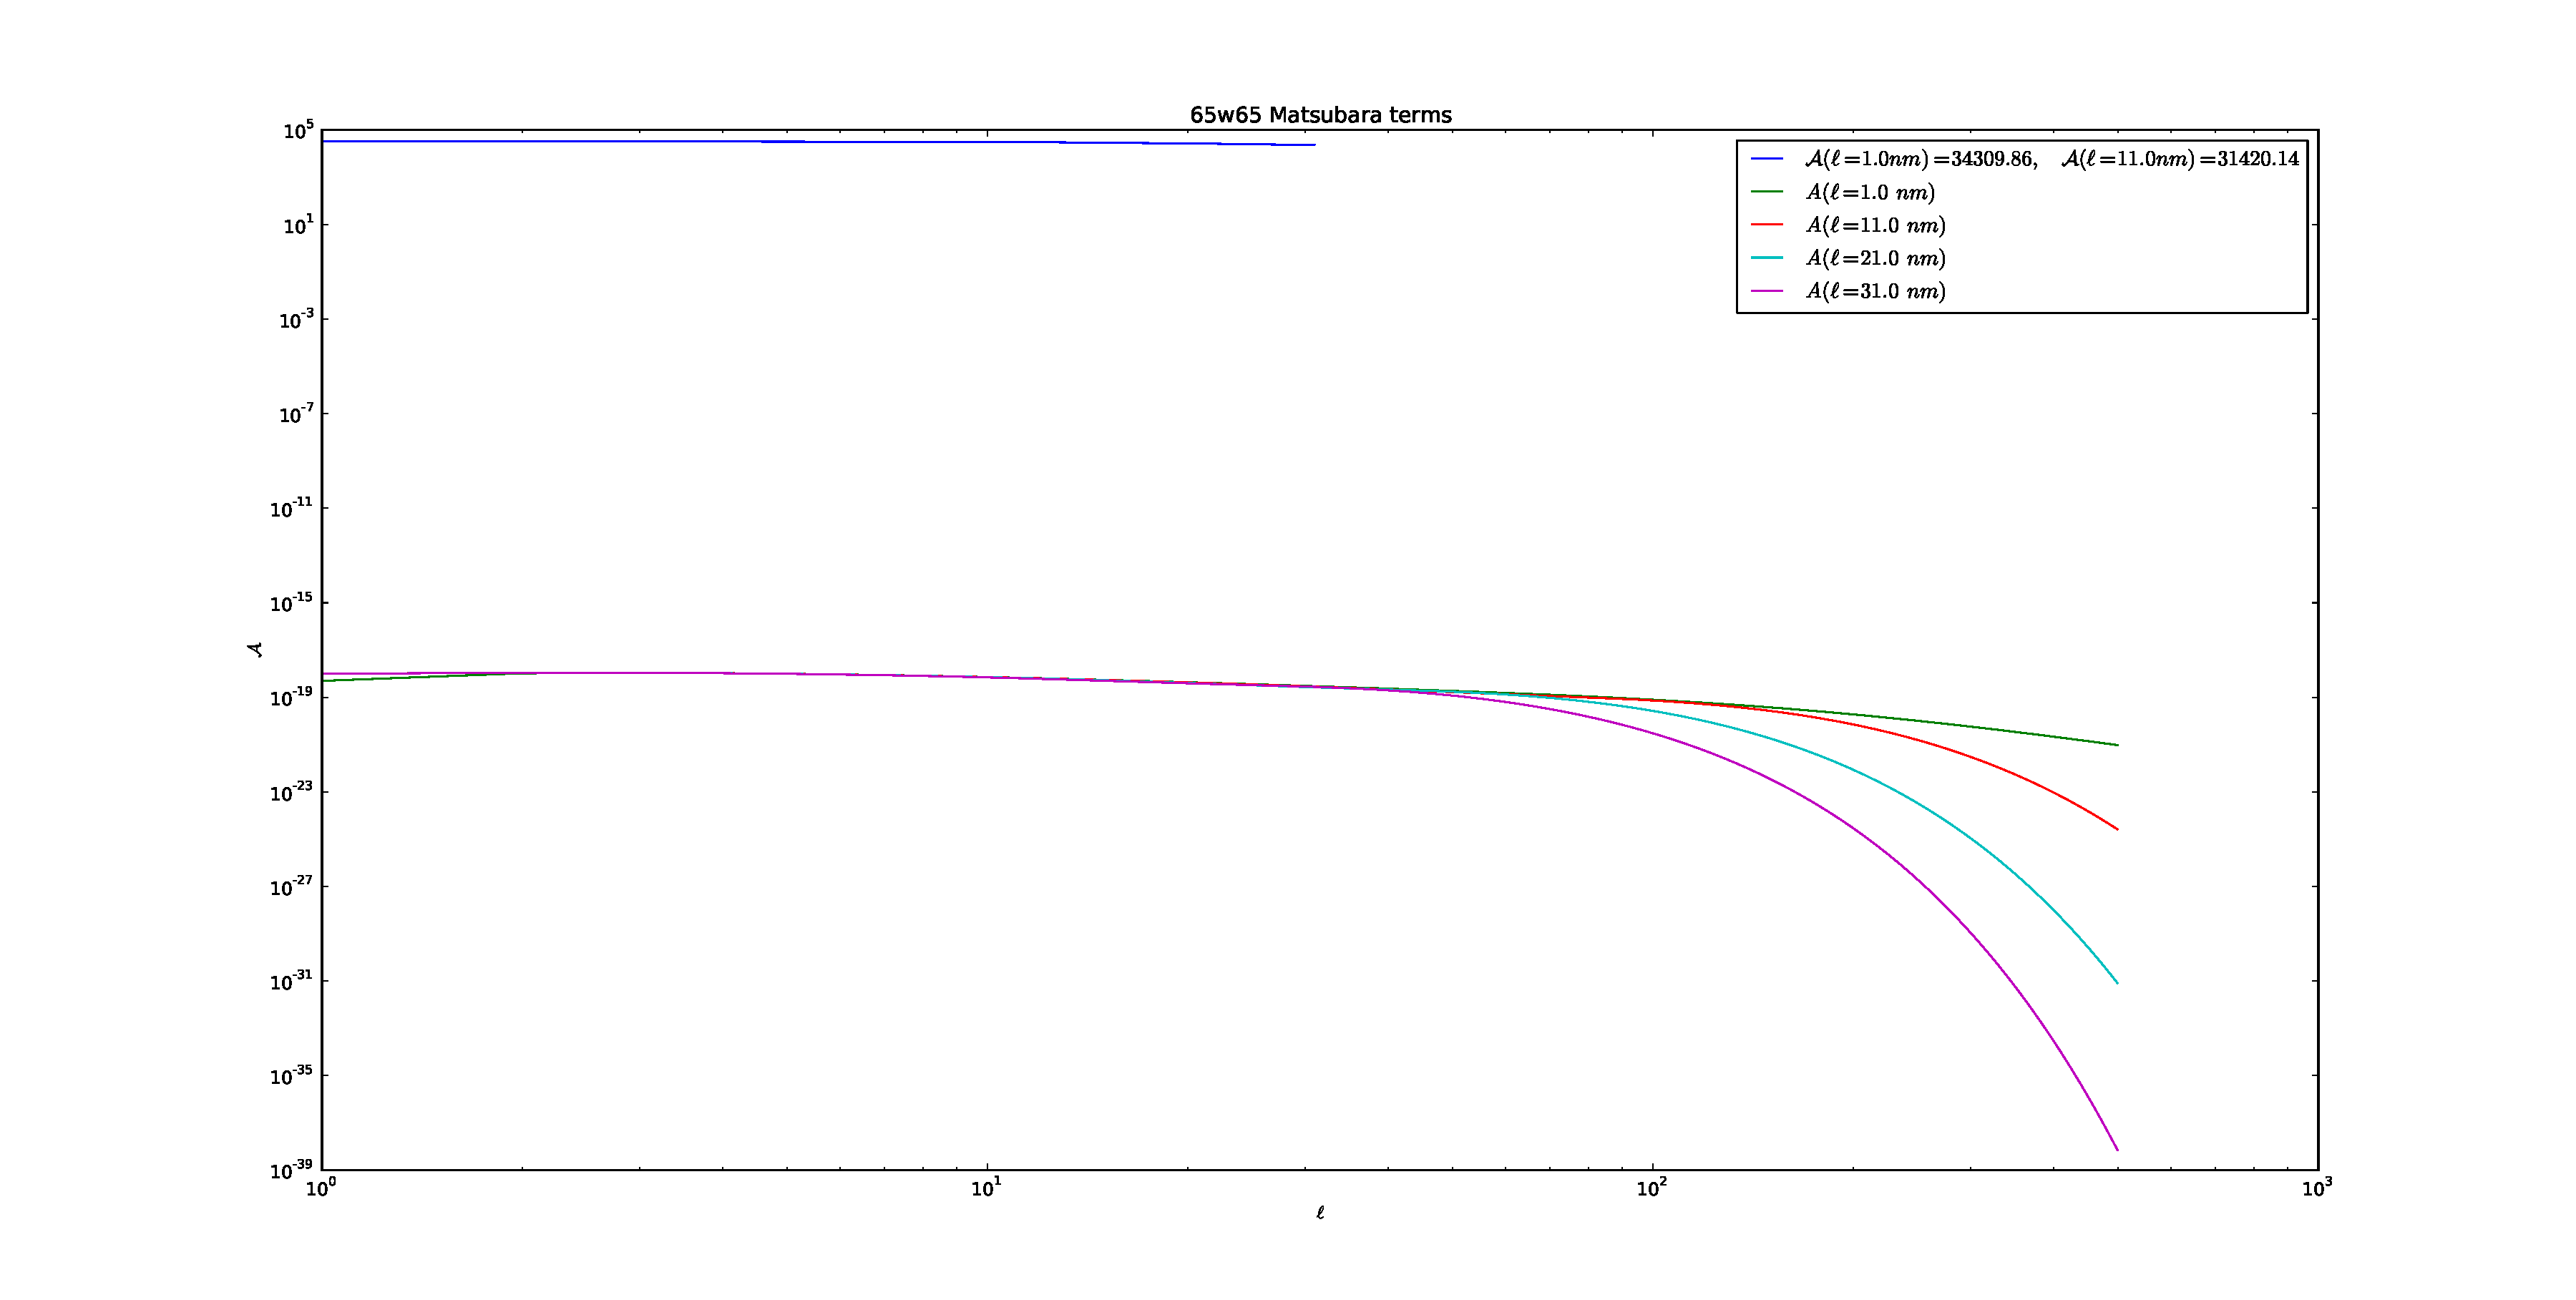
\includegraphics[width=8cm]{par_plots/65w65_A_vs_n.pdf}}%{140309_65w65_GH_skew_ret_A0_A2.pdf}}
%\epsfig {file=sketch.pdf,width=5cm}}
\caption{A sketch of the system of interest (the two cylinders). The quantities describing the geometry of the system are 
denoted, together with the logitudinal and transverse directions of cylinder in the left half-space (1). The skew angle $\theta$ is about an axis normal to the planar boundary defining the limits of each half-space.
}
\label{fig:sketch}
\end{figure}

\begin{figure}
\centerline{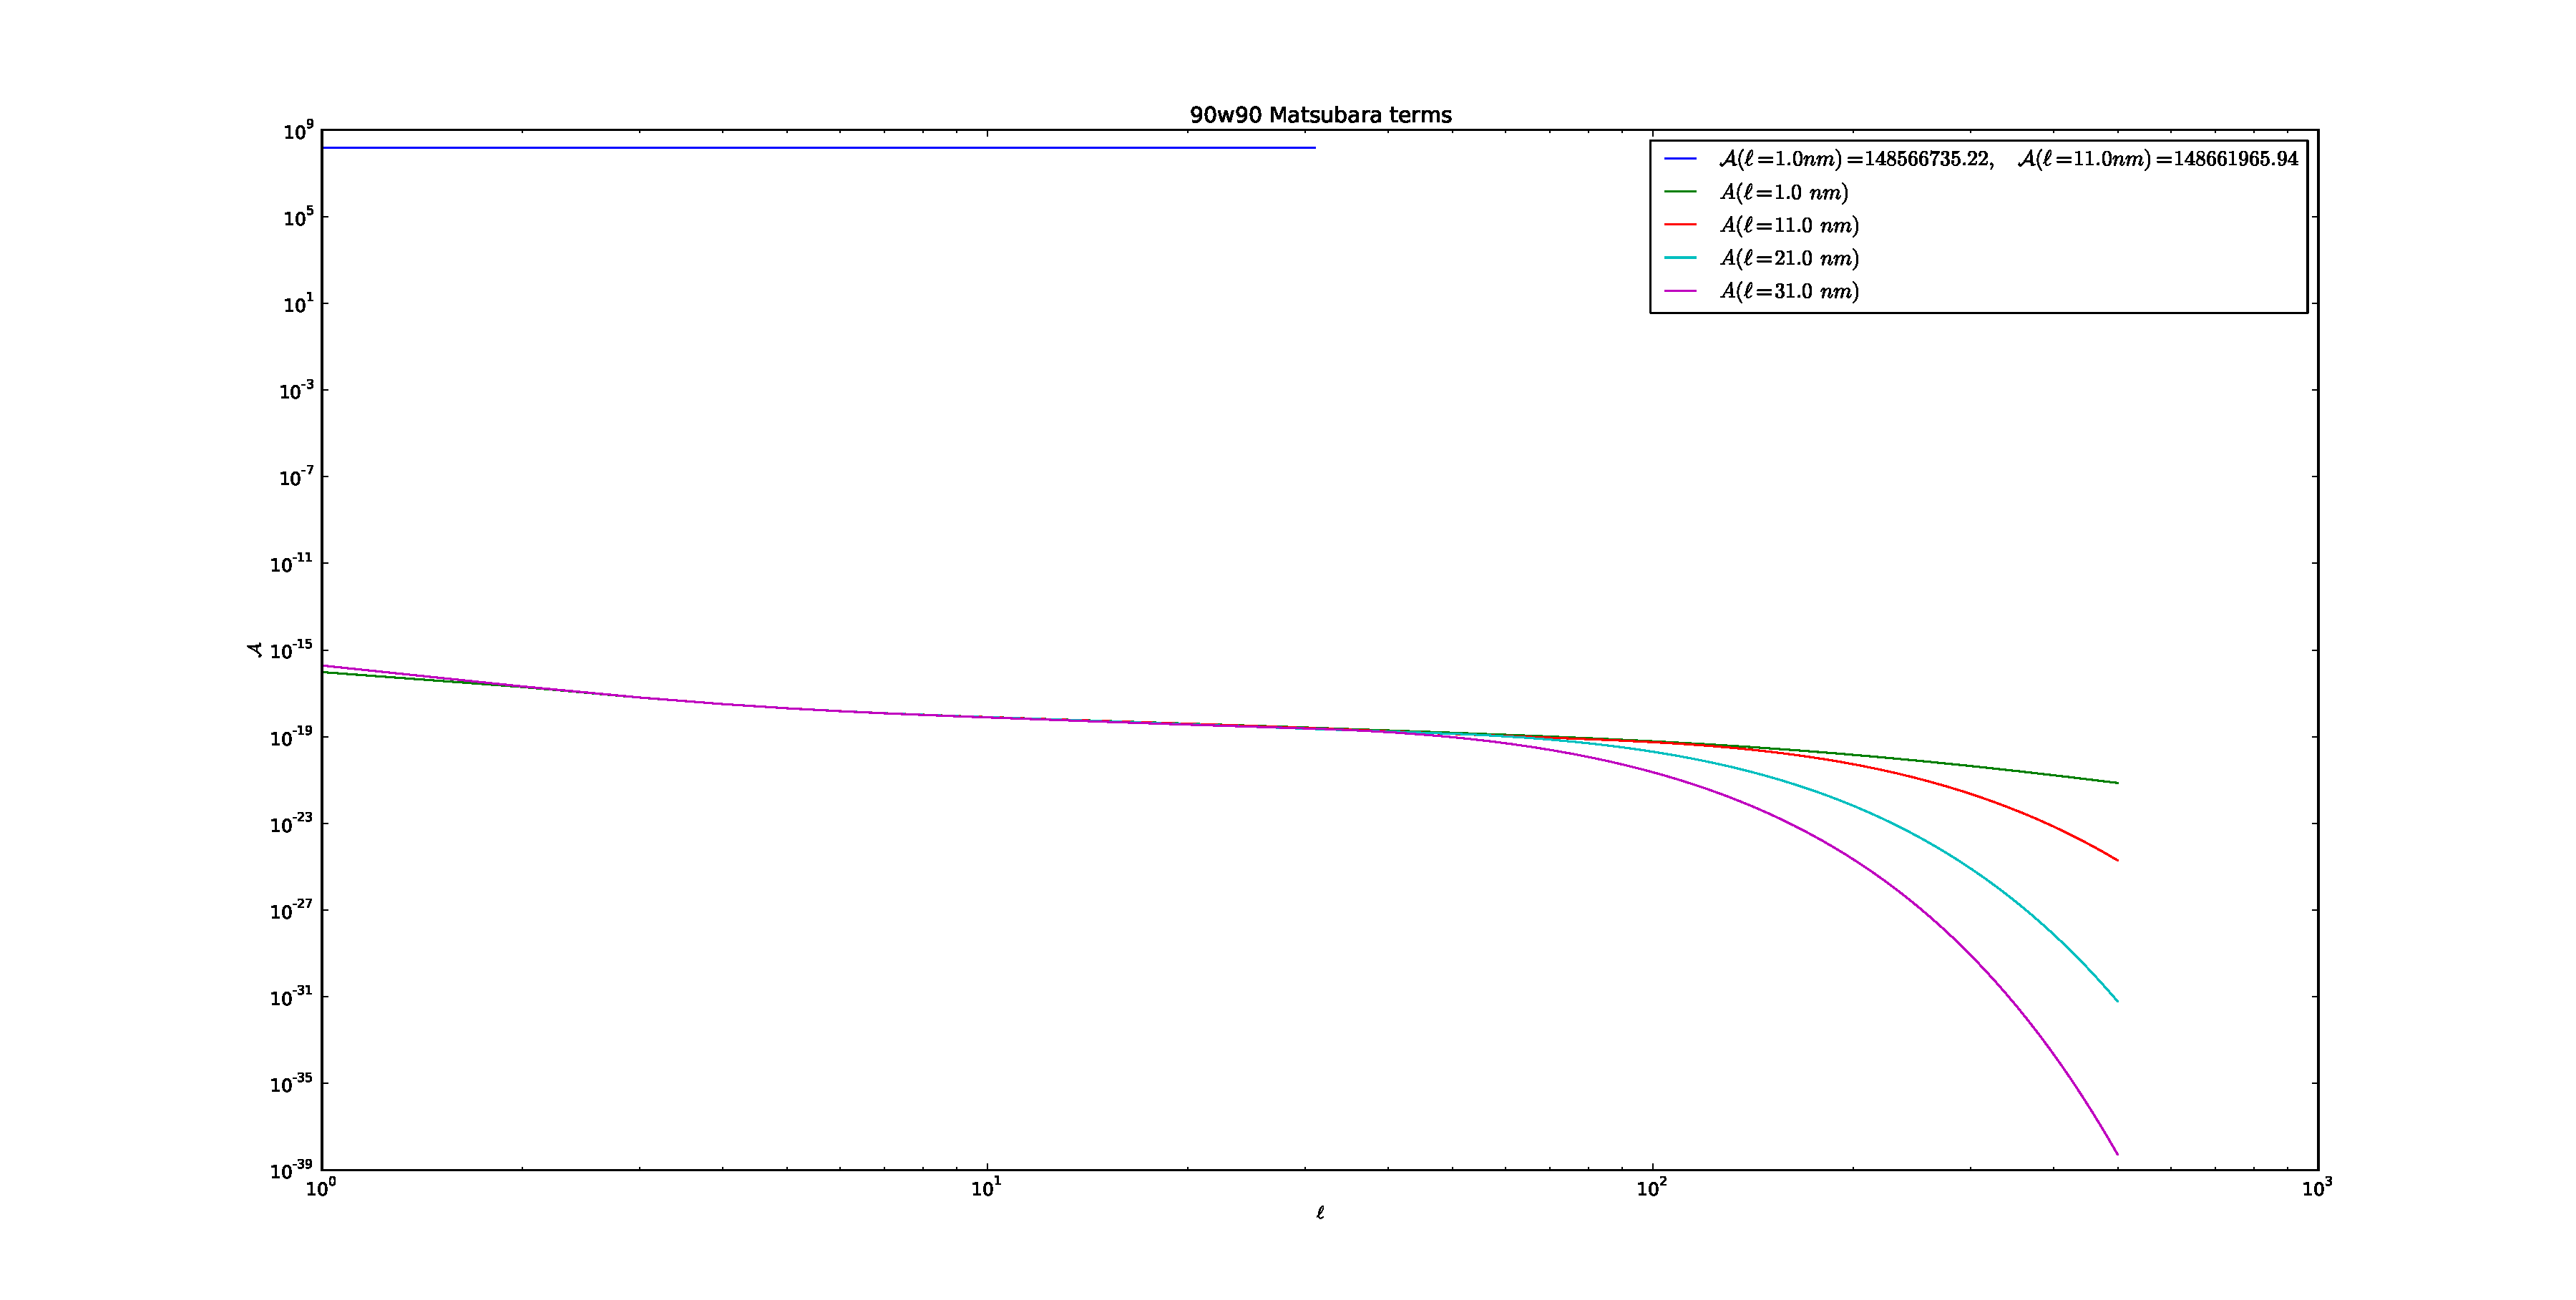
\includegraphics[width=8cm]{par_plots/90w90_A_vs_n.pdf}}%{140309_91w91_GH_skew_ret_A0_A2.pdf}}
%\epsfig {file=sketch.pdf,width=5cm}}
\caption{A sketch of the system of interest (the two cylinders). The quantities describing the geometry of the system are 
denoted, together with the logitudinal and transverse directions of cylinder in the left half-space (1). The skew angle $\theta$ is about an axis normal to the planar boundary defining the limits of each half-space.
}
\label{fig:sketch}
\end{figure}

\begin{figure}
\centerline{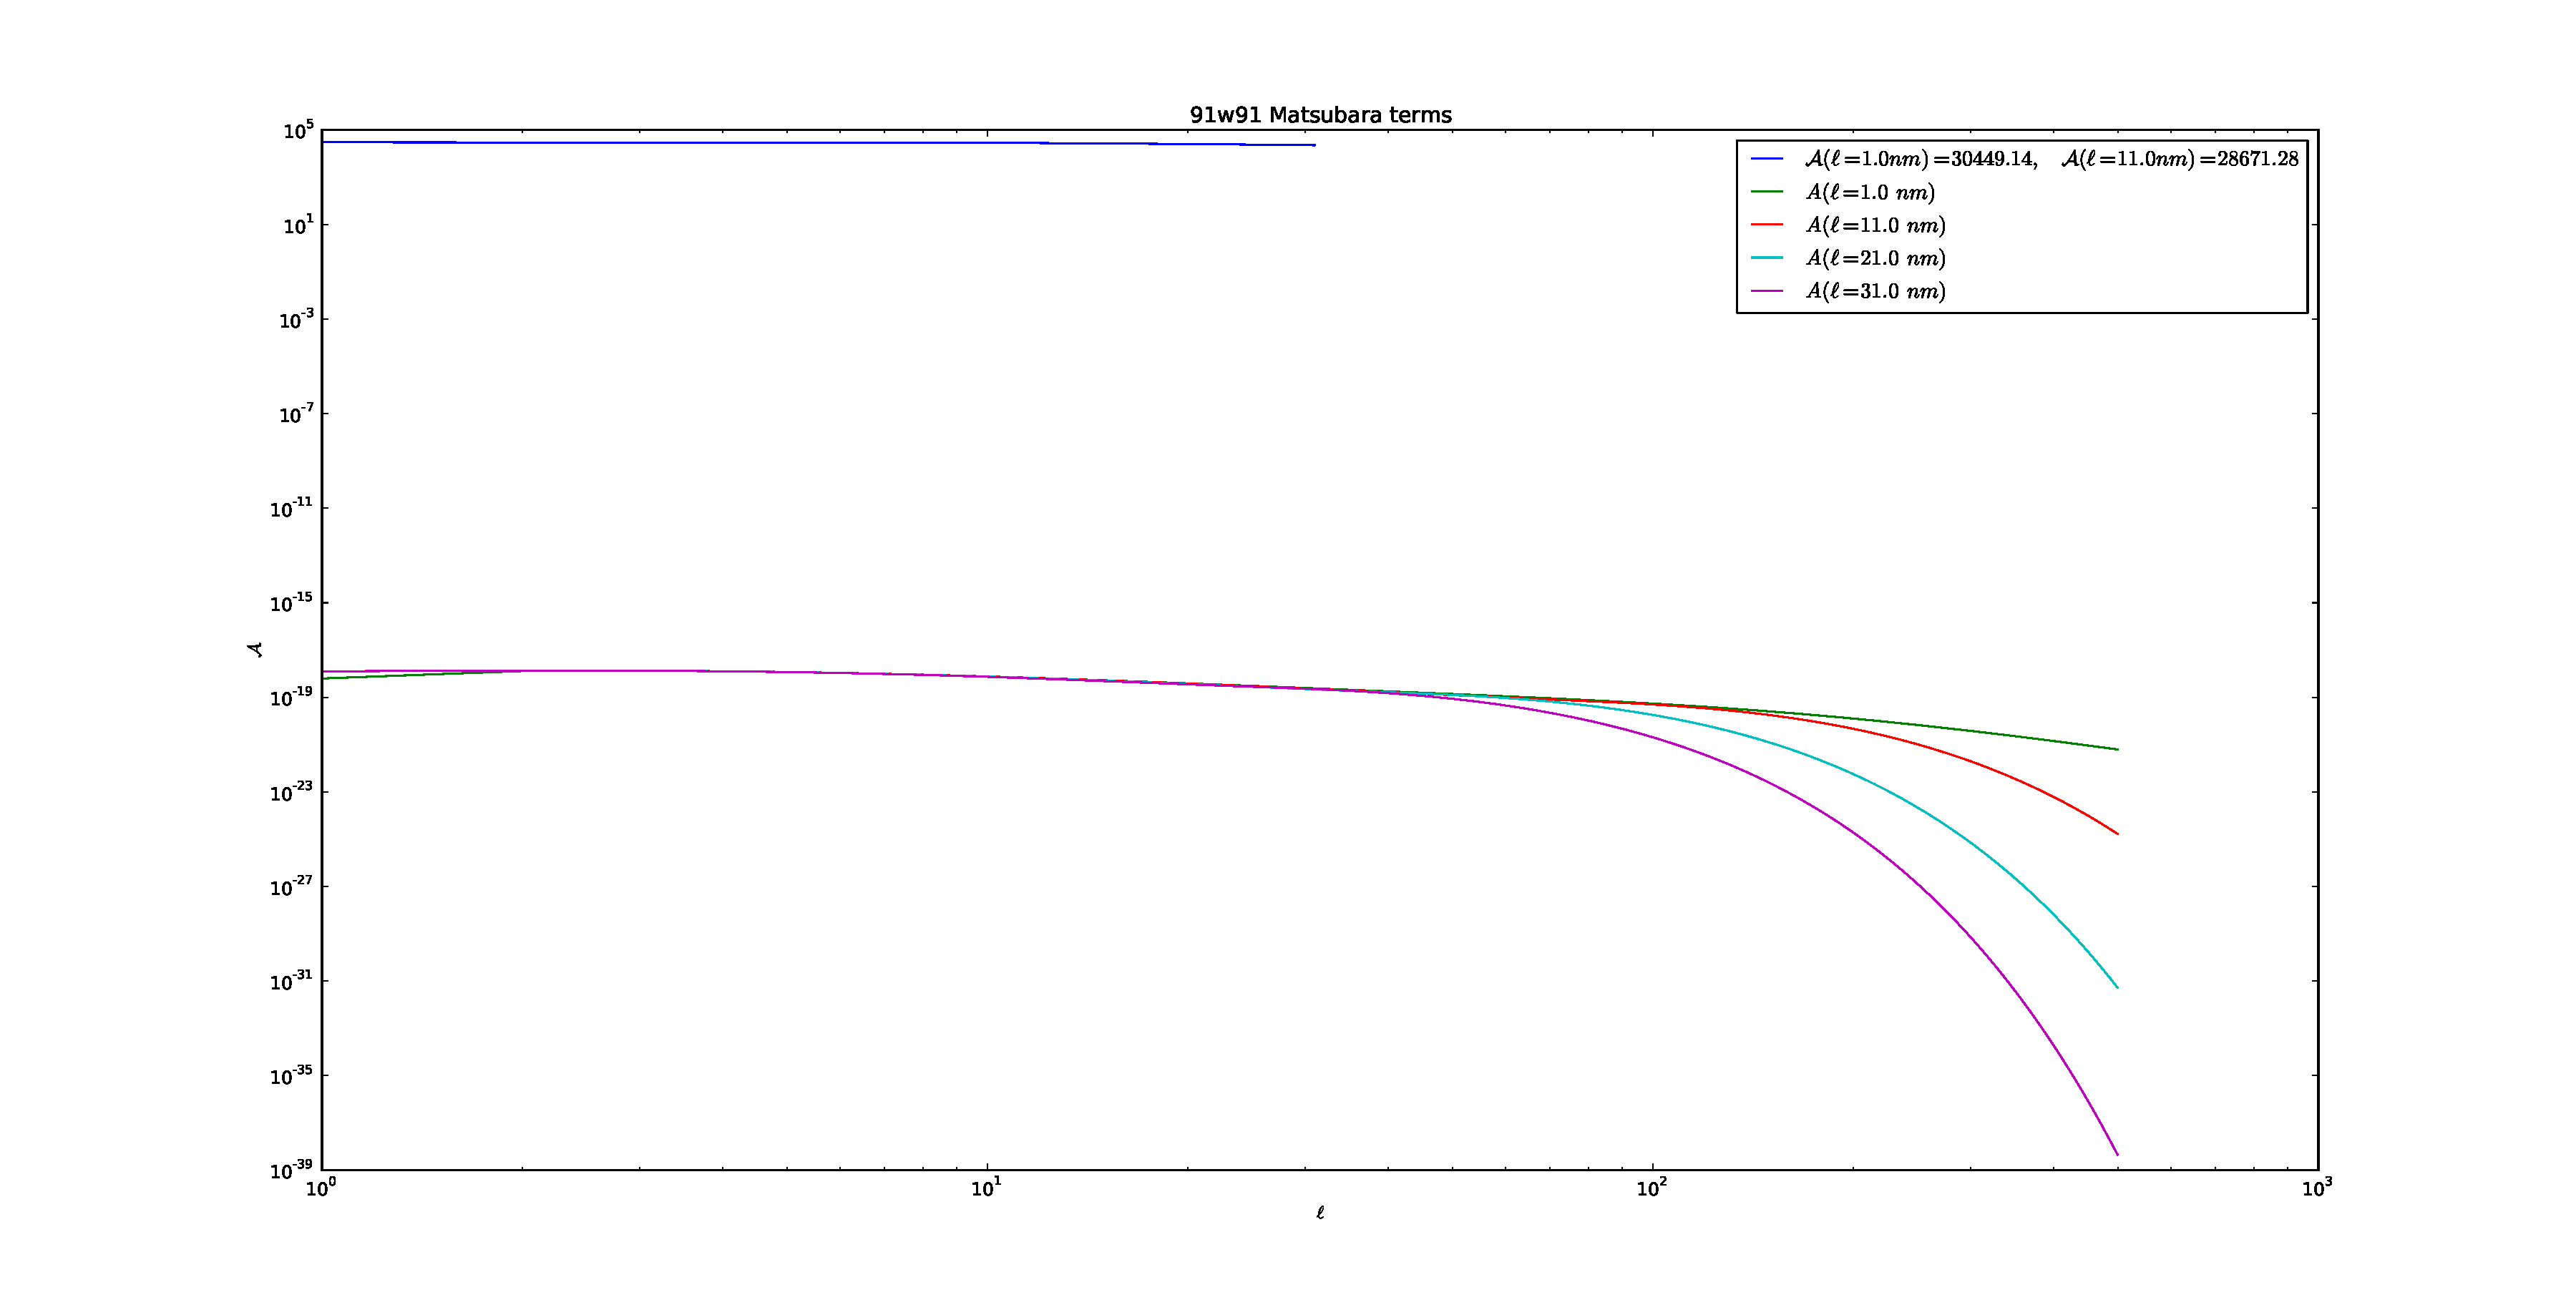
\includegraphics[width=8cm]{par_plots/91w91_A_vs_n.pdf}}%{140309_93w93_GH_skew_ret_A0_A2.pdf}}
%\epsfig {file=sketch.pdf,width=5cm}}
\caption{A sketch of the system of interest (the two cylinders). The quantities describing the geometry of the system are 
denoted, together with the logitudinal and transverse directions of cylinder in the left half-space (1). The skew angle $\theta$ is about an axis normal to the planar boundary defining the limits of each half-space.
}
\label{fig:sketch}
\end{figure}

\begin{figure}
\centerline{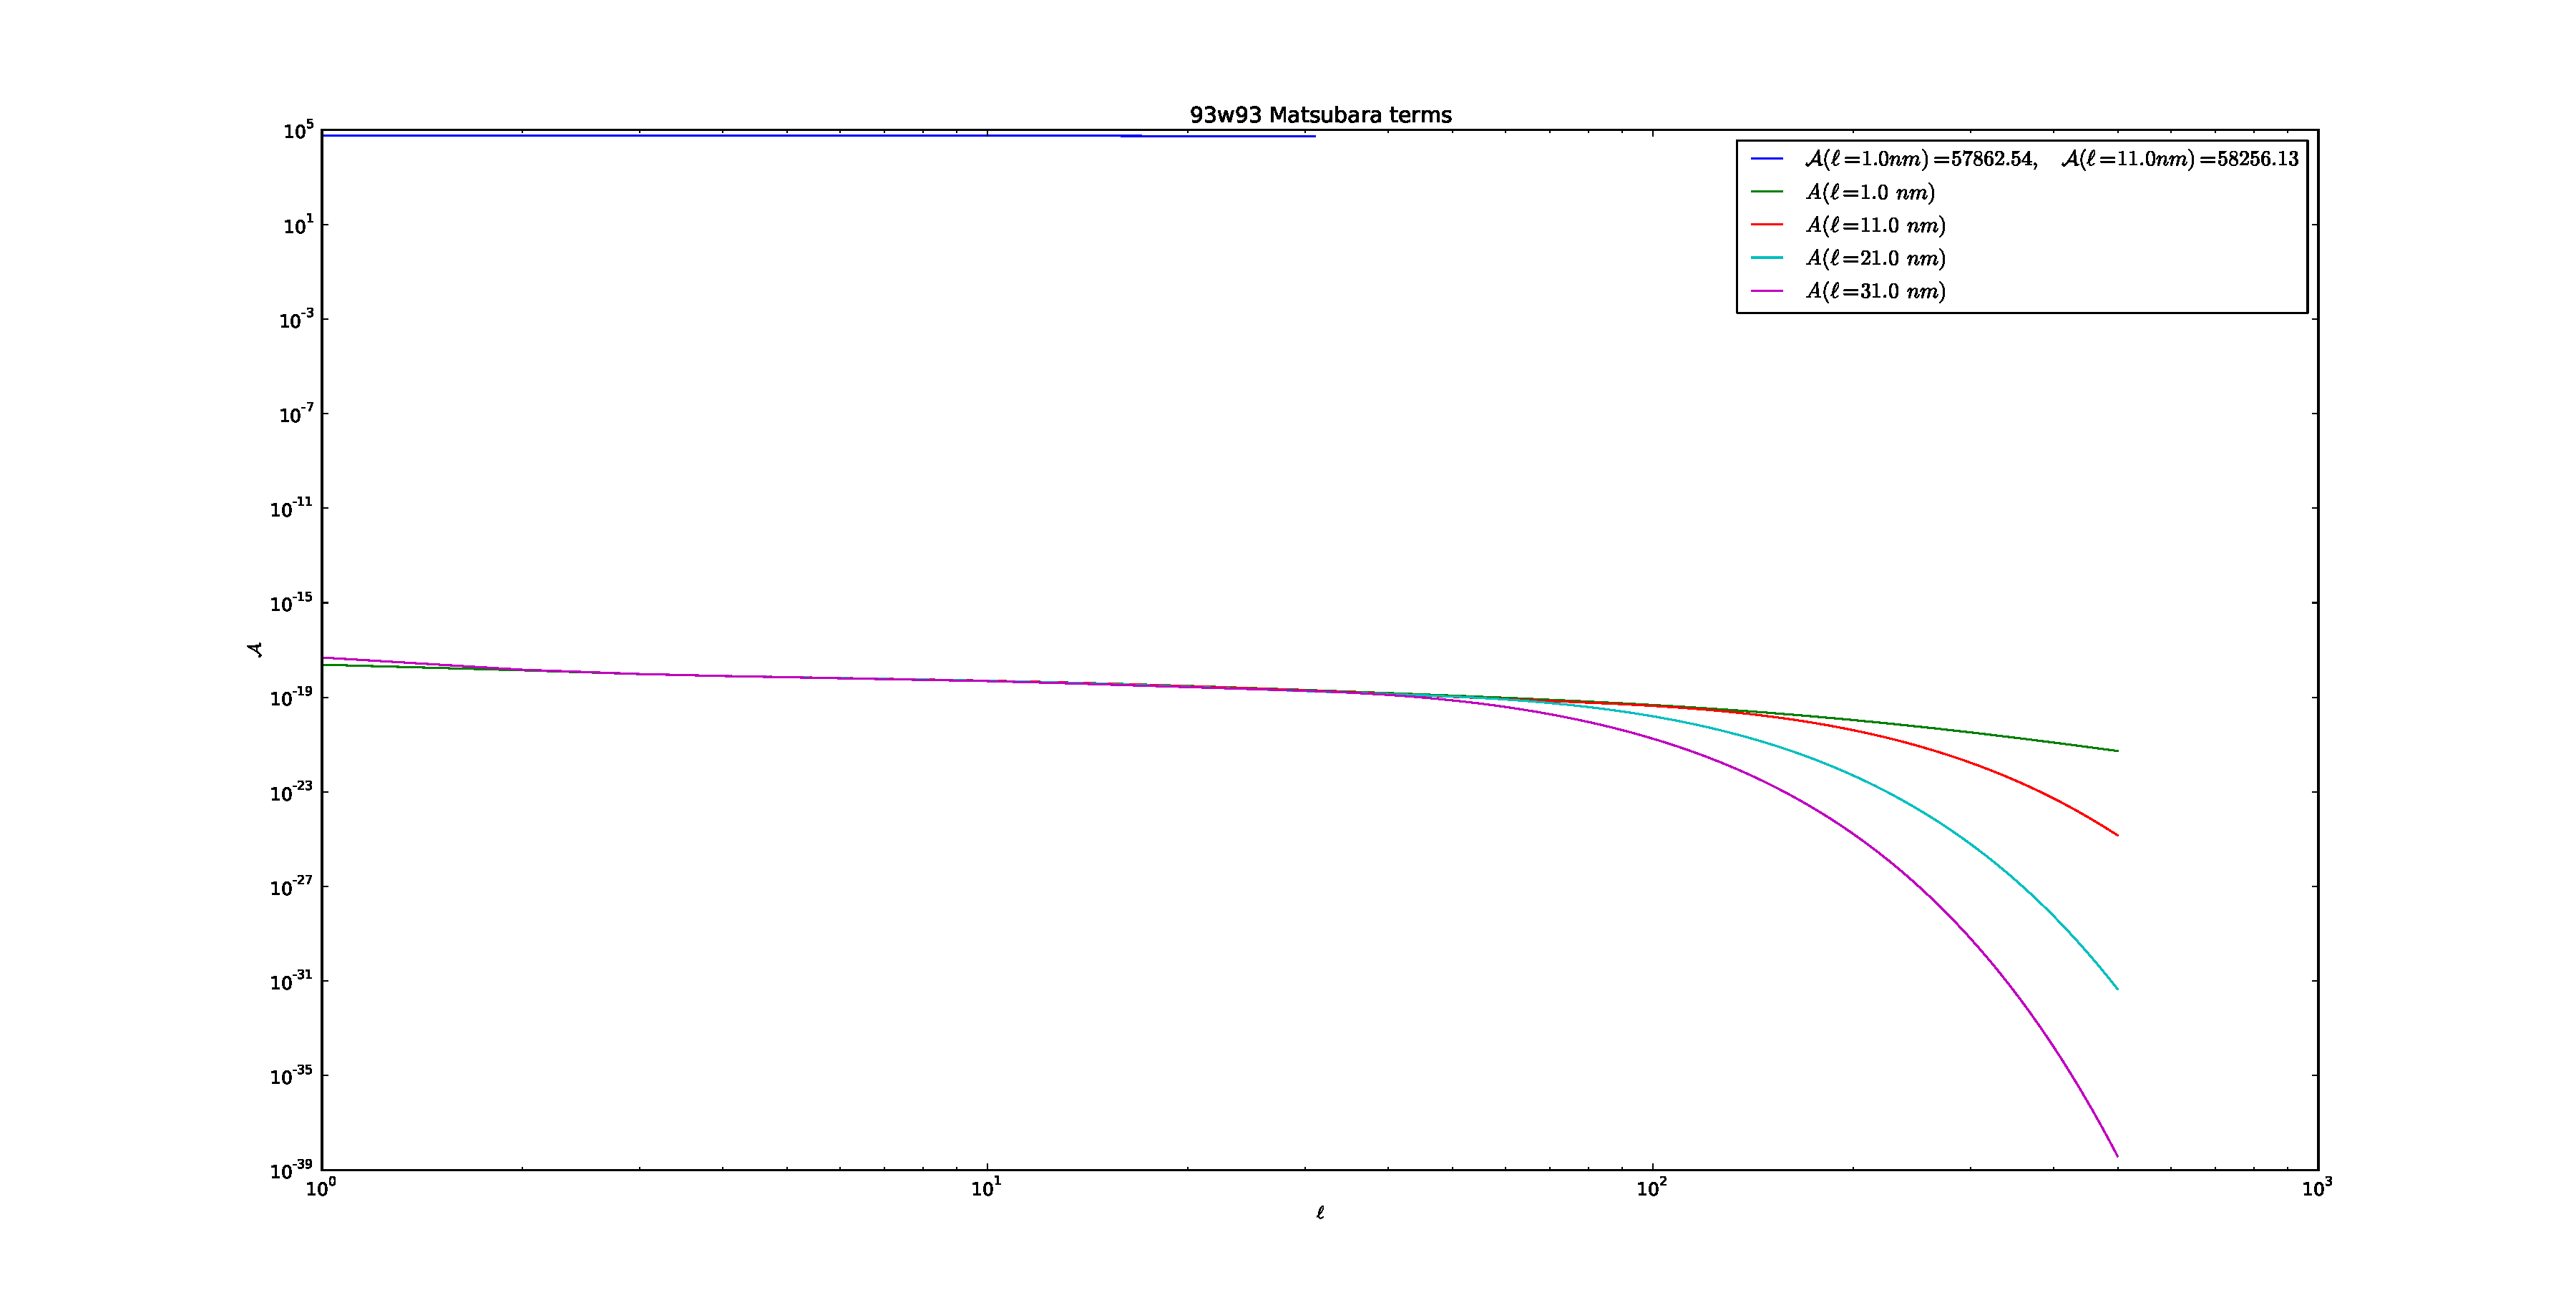
\includegraphics[width=8cm]{par_plots/93w93_A_vs_n.pdf}}%{140309_290w290_GH_skew_ret_A0_A2.pdf}}
%\epsfig {file=sketch.pdf,width=5cm}}
\caption{A sketch of the system of interest (the two cylinders). The quantities describing the geometry of the system are 
denoted, together with the logitudinal and transverse directions of cylinder in the left half-space (1). The skew angle $\theta$ is about an axis normal to the planar boundary defining the limits of each half-space.
}
\label{fig:sketch}
\end{figure}

\begin{figure}
\centerline{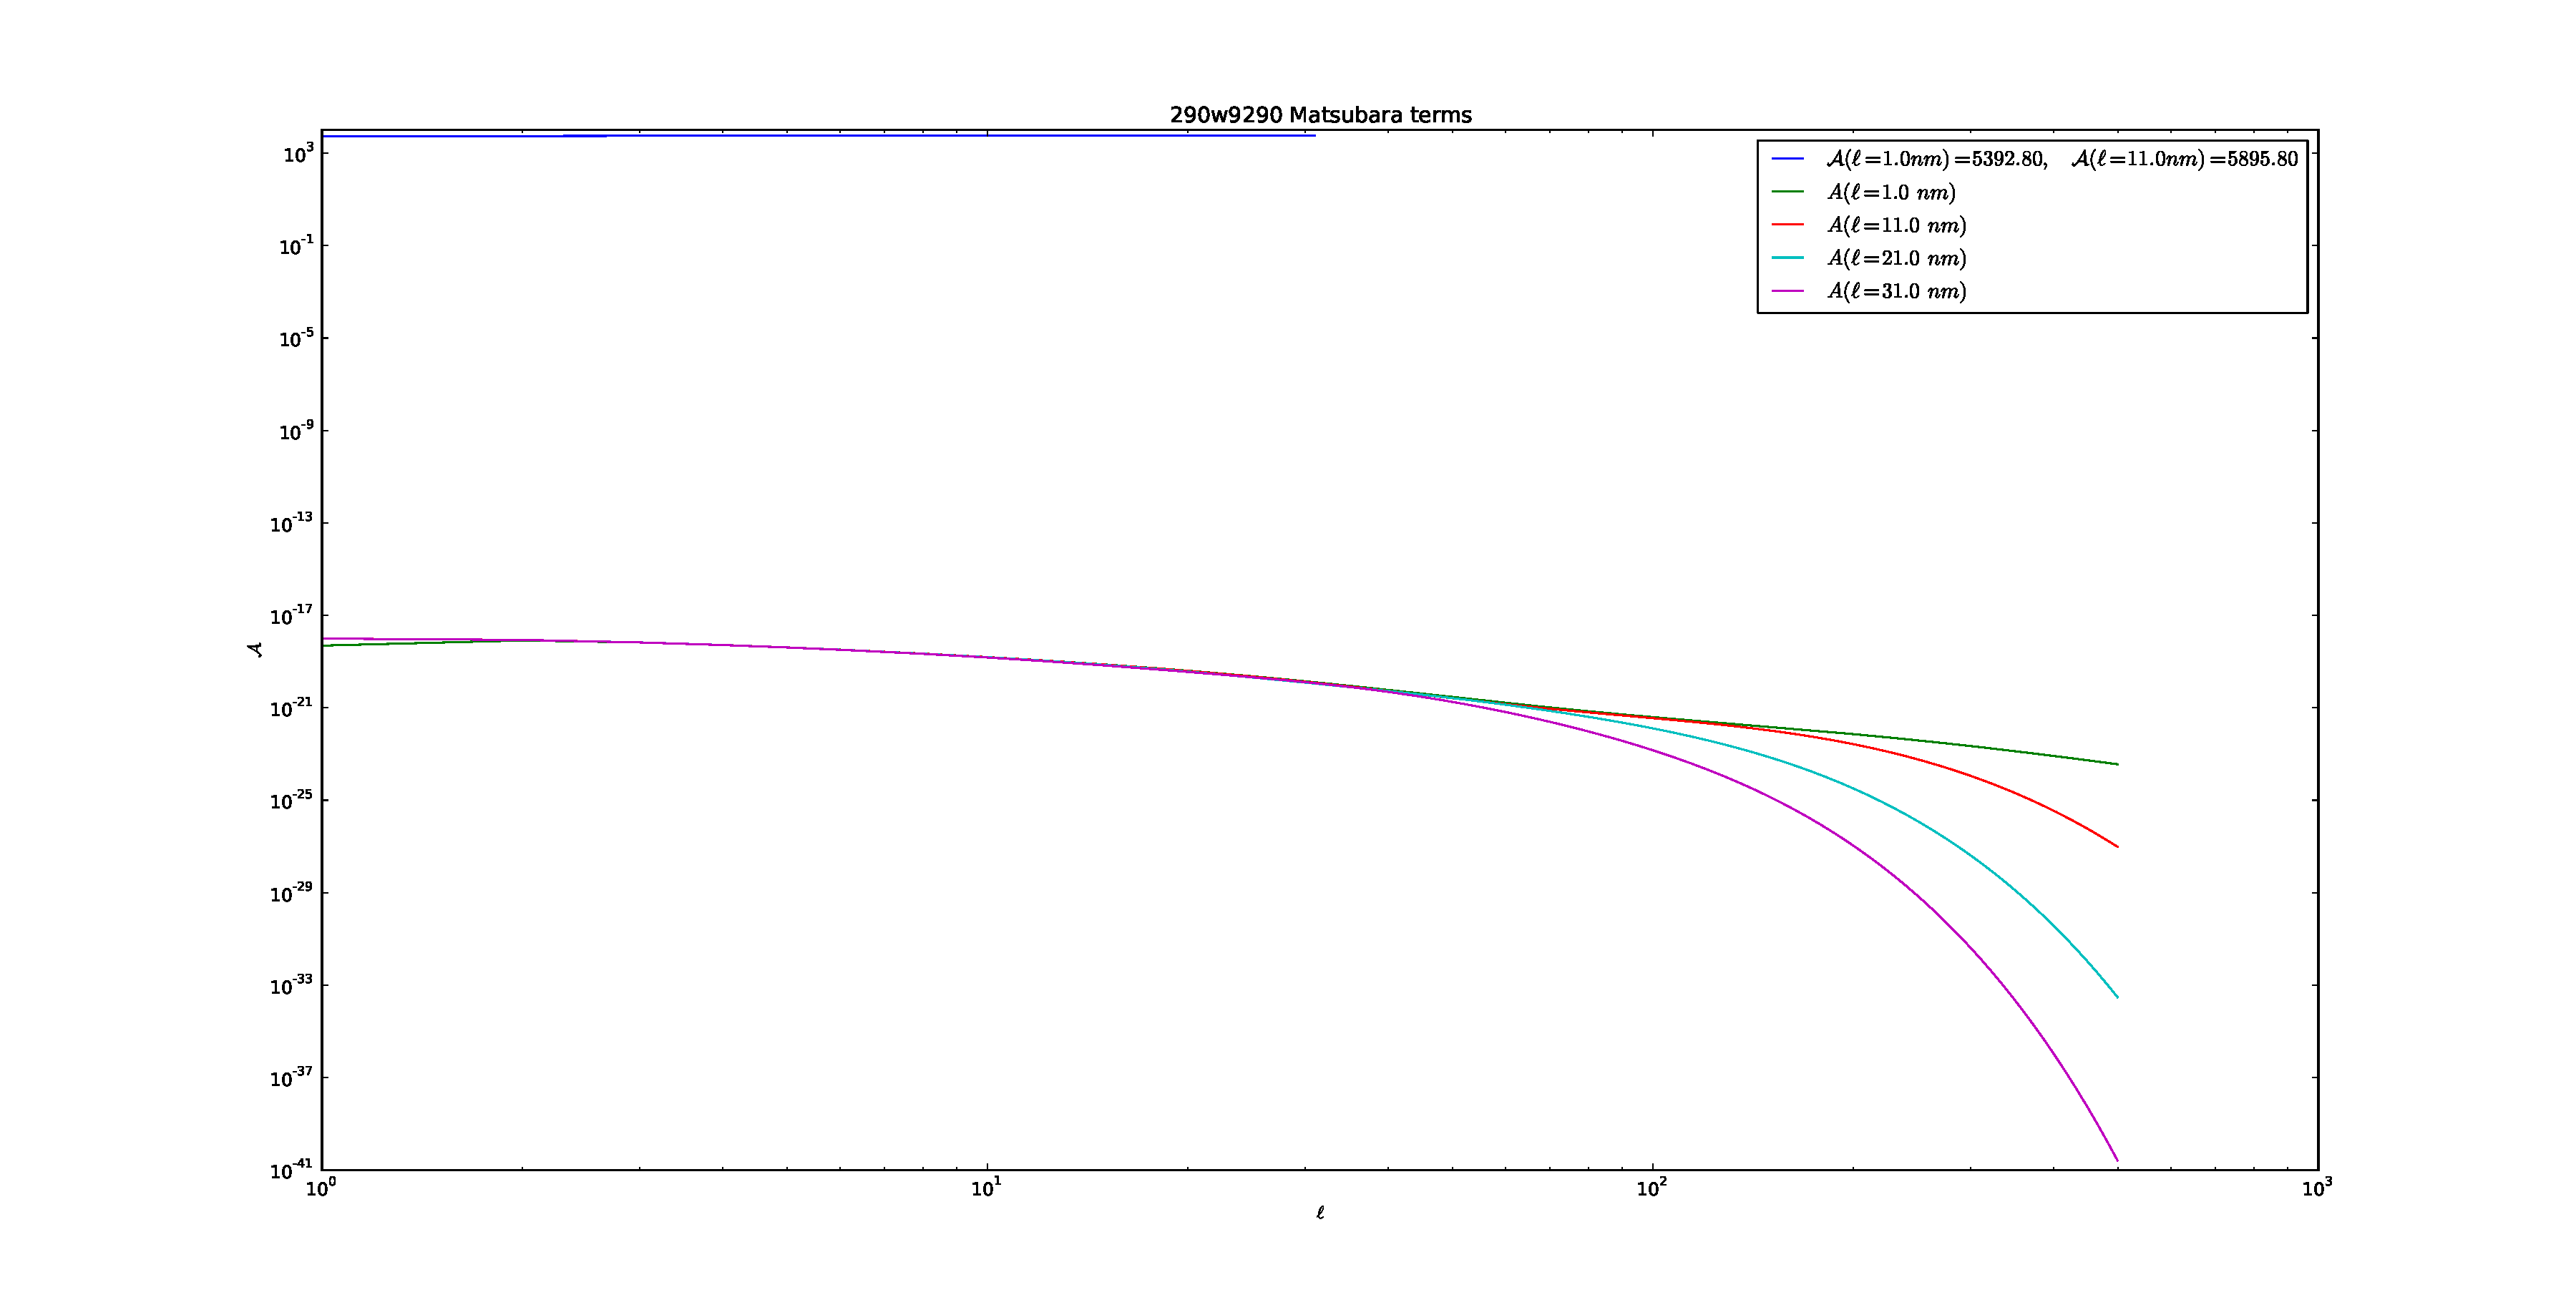
\includegraphics[width=8cm]{par_plots/290w290_A_vs_n.pdf}}%{140309_290w290_GH_skew_ret_A0_A2.pdf}}
%\epsfig {file=sketch.pdf,width=5cm}}
\caption{A sketch of the system of interest (the two cylinders). The quantities describing the geometry of the system are 
denoted, together with the logitudinal and transverse directions of cylinder in the left half-space (1). The skew angle $\theta$ is about an axis normal to the planar boundary defining the limits of each half-space.
}
\label{fig:sketch}
\end{figure}

\begin{table}[ht]
\caption{Hamaker coefficents for parallel cylinders, retarded formulation at
intersurface distance of 1 nm}% title of Table
\centering
% used for centering table
\begin{tabular}{r c | l | l}
  \hline                       
  & CNT & $\mathcal{A}^{0}$ [zJ] & 3$\mathcal{A}^{2}$ [zJ] \\
  \hline
  &[6,5]  & 105.46 & 0.96 \\
  &[9,0]  & addressing & monopole flucuations \\
  &[9,1]  & 93.56 & 1.56 \\
  &[9,3]  & addressing & monopole flucuations \\
  &[29,0] & 17.73 & 0.41 \\
  \hline  
\end{tabular}
\label{table:nonlin}
% is used to refer this table in the text

\end{table}


\begin{table}[ht]
\caption{Hamaker coefficents for parallel cylinders, Non-retarded formulation}% title of Table
\centering
% used for centering table
\begin{tabular}{r c | l | l}
  \hline                       
  & CNT & $\mathcal{A}^{0}$ [zJ] & 3$\mathcal{A}^{2}$ [zJ] \\
  \hline
  &[6,5]  & 105.46 & 0.96 \\
  &[9,0]  & addressing & monopole flucuations \\
  &[9,1]  & 93.56 & 1.56 \\
  &[9,3]  & addressing & monopole flucuations \\
  &[29,0] & 17.73 & 0.41 \\
  \hline  
\end{tabular}
\label{table:nonlin}
% is used to refer this table in the text

\end{table}



\end{document}


